% !TeX program = pdflatex
% Multi-Agent World, ICLR 2027 submission.
% This file is the revised manuscript. The original draft remains in
% iclr2027_conference.tex and sections/ and is not modified.
\documentclass{article}

\usepackage{iclr2027_conference, times}

\input{math_commands.tex}

\usepackage{amsmath}
\usepackage{amssymb}
\usepackage{algorithm}
\usepackage{algorithmic}
\usepackage{graphicx}
\usepackage{booktabs}
\usepackage{tabularx}
\usepackage{array}
\usepackage{multirow}
\usepackage{colortbl}
\usepackage{xcolor}
\usepackage{enumitem}
\usepackage{microtype}
\usepackage{placeins}
\usepackage[most]{tcolorbox}
\usepackage{listings}
\usepackage{float}
\usepackage{hyperref}
\hypersetup{hidelinks}
\graphicspath{{figures/}}

% ---------------------------------------------------------------------------
% Shorthands
% ---------------------------------------------------------------------------
\newcommand{\maw}{\textsc{MAW}}
\newcommand{\up}{$\uparrow$}
\newcommand{\down}{$\downarrow$}
% Slot for a measurement that the authors fill in after the final runs.
\newcommand{\fillin}{\underline{\hspace{1.6em}}}

\newcolumntype{Y}{>{\raggedright\arraybackslash}X}
\newcolumntype{C}[1]{>{\centering\arraybackslash}p{#1}}

% Case cards in the appendix.
\definecolor{caseink}{HTML}{243748}
\definecolor{caseteal}{HTML}{398F84}
\newtcolorbox{systembox}[1]{enhanced,breakable,
  colback=white,colframe=caseink!65!white,
  colbacktitle=caseink,coltitle=white,
  title={#1},fonttitle=\sffamily\bfseries,fontupper=\small,
  boxrule=0.5pt,arc=1mm,left=3mm,right=3mm,top=2mm,bottom=2mm,
  before skip=7pt,after skip=6pt}
\newcommand{\casepart}[1]{\par\vspace{5pt}%
  {\color{caseteal!85!black}\sffamily\bfseries #1}\par\nobreak\vspace{3pt}}
\lstdefinestyle{casejson}{basicstyle=\ttfamily\small,
  columns=fullflexible,keepspaces=true,breaklines=true,
  showstringspaces=false,aboveskip=0pt,belowskip=0pt}

\title{Multi-Agent World: Scaling Multi-Agent Orchestration Training\\ via Recursive Environment Improvement and Schedule-Aware Rewards}

\author{Anonymous Authors}

% Uncomment only for the camera-ready version.
% \iclrfinalcopy

\begin{document}
\raggedbottom

\maketitle

\begin{abstract}
Multi-agent systems assign complementary subtasks to different agents, and their effectiveness depends on an orchestrator that partitions a request into subtasks, schedules them against their dependencies, and integrates the evidence that workers return.
Training such an orchestrator requires multi-agent environments, in which a task provides subtasks that can be distributed across agents and a verifier that reports how they were distributed.
Existing agentic environments are synthesized for a single agent, and they yield mostly linear call chains under terminal-only verification.
An orchestrator trained inside them therefore has no scheduling decision to learn and no feedback on the decomposition it chose.
We present \emph{Multi-Agent World} (MAW), an end-to-end framework that develops multi-agent orchestration by coupling multi-agent environment synthesis with multi-agent reinforcement learning.
MAW introduces \emph{recursive environment improvement}, which recursively composes reference task graphs through serial and parallel operators inside single-agent environments, and turns each composed graph into one coherent request through semantic reconstruction and execution-grounded admission.
The same composition record identifies which subtasks are verified as independent, which is what a \emph{schedule-aware process reward} needs in order to score the recorded execution of the whole team.
Trained under this reward with frozen workers, the orchestrator learns to decompose a request, run independent work concurrently, and integrate what the workers return.
Experiments on six agentic benchmarks show that MAW improves task success by \fillin\ over its single-agent initialization and shortens the execution critical path by \fillin.

\end{abstract}

\section{Introduction}
\label{sec:intro}

Large language model (LLM) agents now carry out workflows that combine information gathering, tool use, and multi-step reasoning~\citep{yao2023react,schick2023toolformer,qin2024toolllm}.
Such a workflow usually contains complementary subtasks whose outputs must be assembled into one solution, and multi-agent systems assign each subtask to a separate agent, as exemplified by AutoGen~\citep{wu2023autogenenablingnextgenllm} and MetaGPT~\citep{hong2024metagptmetaprogrammingmultiagent}.
Recent systems further execute independent subtasks concurrently, which shortens the critical path of a long workflow~\citep{anthropic2025multiagent,kimiteam2026kimik25}.
However, distributing a task across agents does not by itself produce a better solution.
The benefit instead depends on three decisions, namely how the request is divided, when each part is executed, and how the returned results are combined.
In a multi-agent system, one component makes all three, the orchestrator.

Building an effective multi-agent system is difficult, as these three decisions constrain one another.
An ideal orchestrator first partitions a request into subtasks that one worker can finish alone.
Subtasks that are too fine raise the coordination overhead, while subtasks that are too coarse reduce the team to a single agent.
The orchestrator then separates the subtasks that consume the output of another subtask from the subtasks that are genuinely independent.
For instance, a request that compares several vendors can retrieve each vendor in parallel, while the comparison itself must wait for every retrieval to return.
While treating a dependent subtask as independent lets a worker execute on incomplete information, treating an independent subtask as dependent serializes work that could have progressed concurrently.
Throughout, the orchestrator never accesses a tool or a record itself.
A single agent inspects one observation and corrects its next call.
In contrast, the orchestrator observes only what workers report and therefore commits to a decomposition before any evidence exists.
Therefore, an orchestrator learns this capability from multi-agent interaction and not from a collaboration procedure fixed in advance.

In most multi-agent systems, orchestration is still designed by hand, as in AutoGen and MetaGPT, where roles, routes, and execution order are fixed in a predefined workflow and the model operates within a collaboration structure that it does not determine.
A recent line of work does train orchestration with reinforcement learning~\citep{kimiteam2026kimik25,yuan2026paramanager,dang2025puppeteer}, which establishes that the capability is learnable.
Scaling that training is limited by the environments available for learning.
Specifically, a multi-agent environment offers a task whose subtasks can be distributed across agents, together with a verifier reporting how the team distributed them.
Current environment synthesis provides neither property, as AWM~\citep{wang2026agentworldmodelinfinity}, EnvScaler~\citep{song2026envscaler}, Agent-World~\citep{dong2026agentworld} and ToolVerse~\citep{zhou2026toolverse} build code-backed environments for a single agent that observes every tool return itself.
A task synthesized this way is usually one chain of calls in which every step consumes the previous observation.
In essence, single-agent environments and multi-agent environments differ in two ways.
First, a single-agent task carries no controlled branch structure, thereby leaving an orchestrator with no scheduling decision to practice.
Second, a single-agent task is scored only by terminal success.
Under such a score, a team that partitions the work correctly and misses one integration step is indistinguishable from a team that never decomposes the request.

\begin{figure}[t]
  \centering
  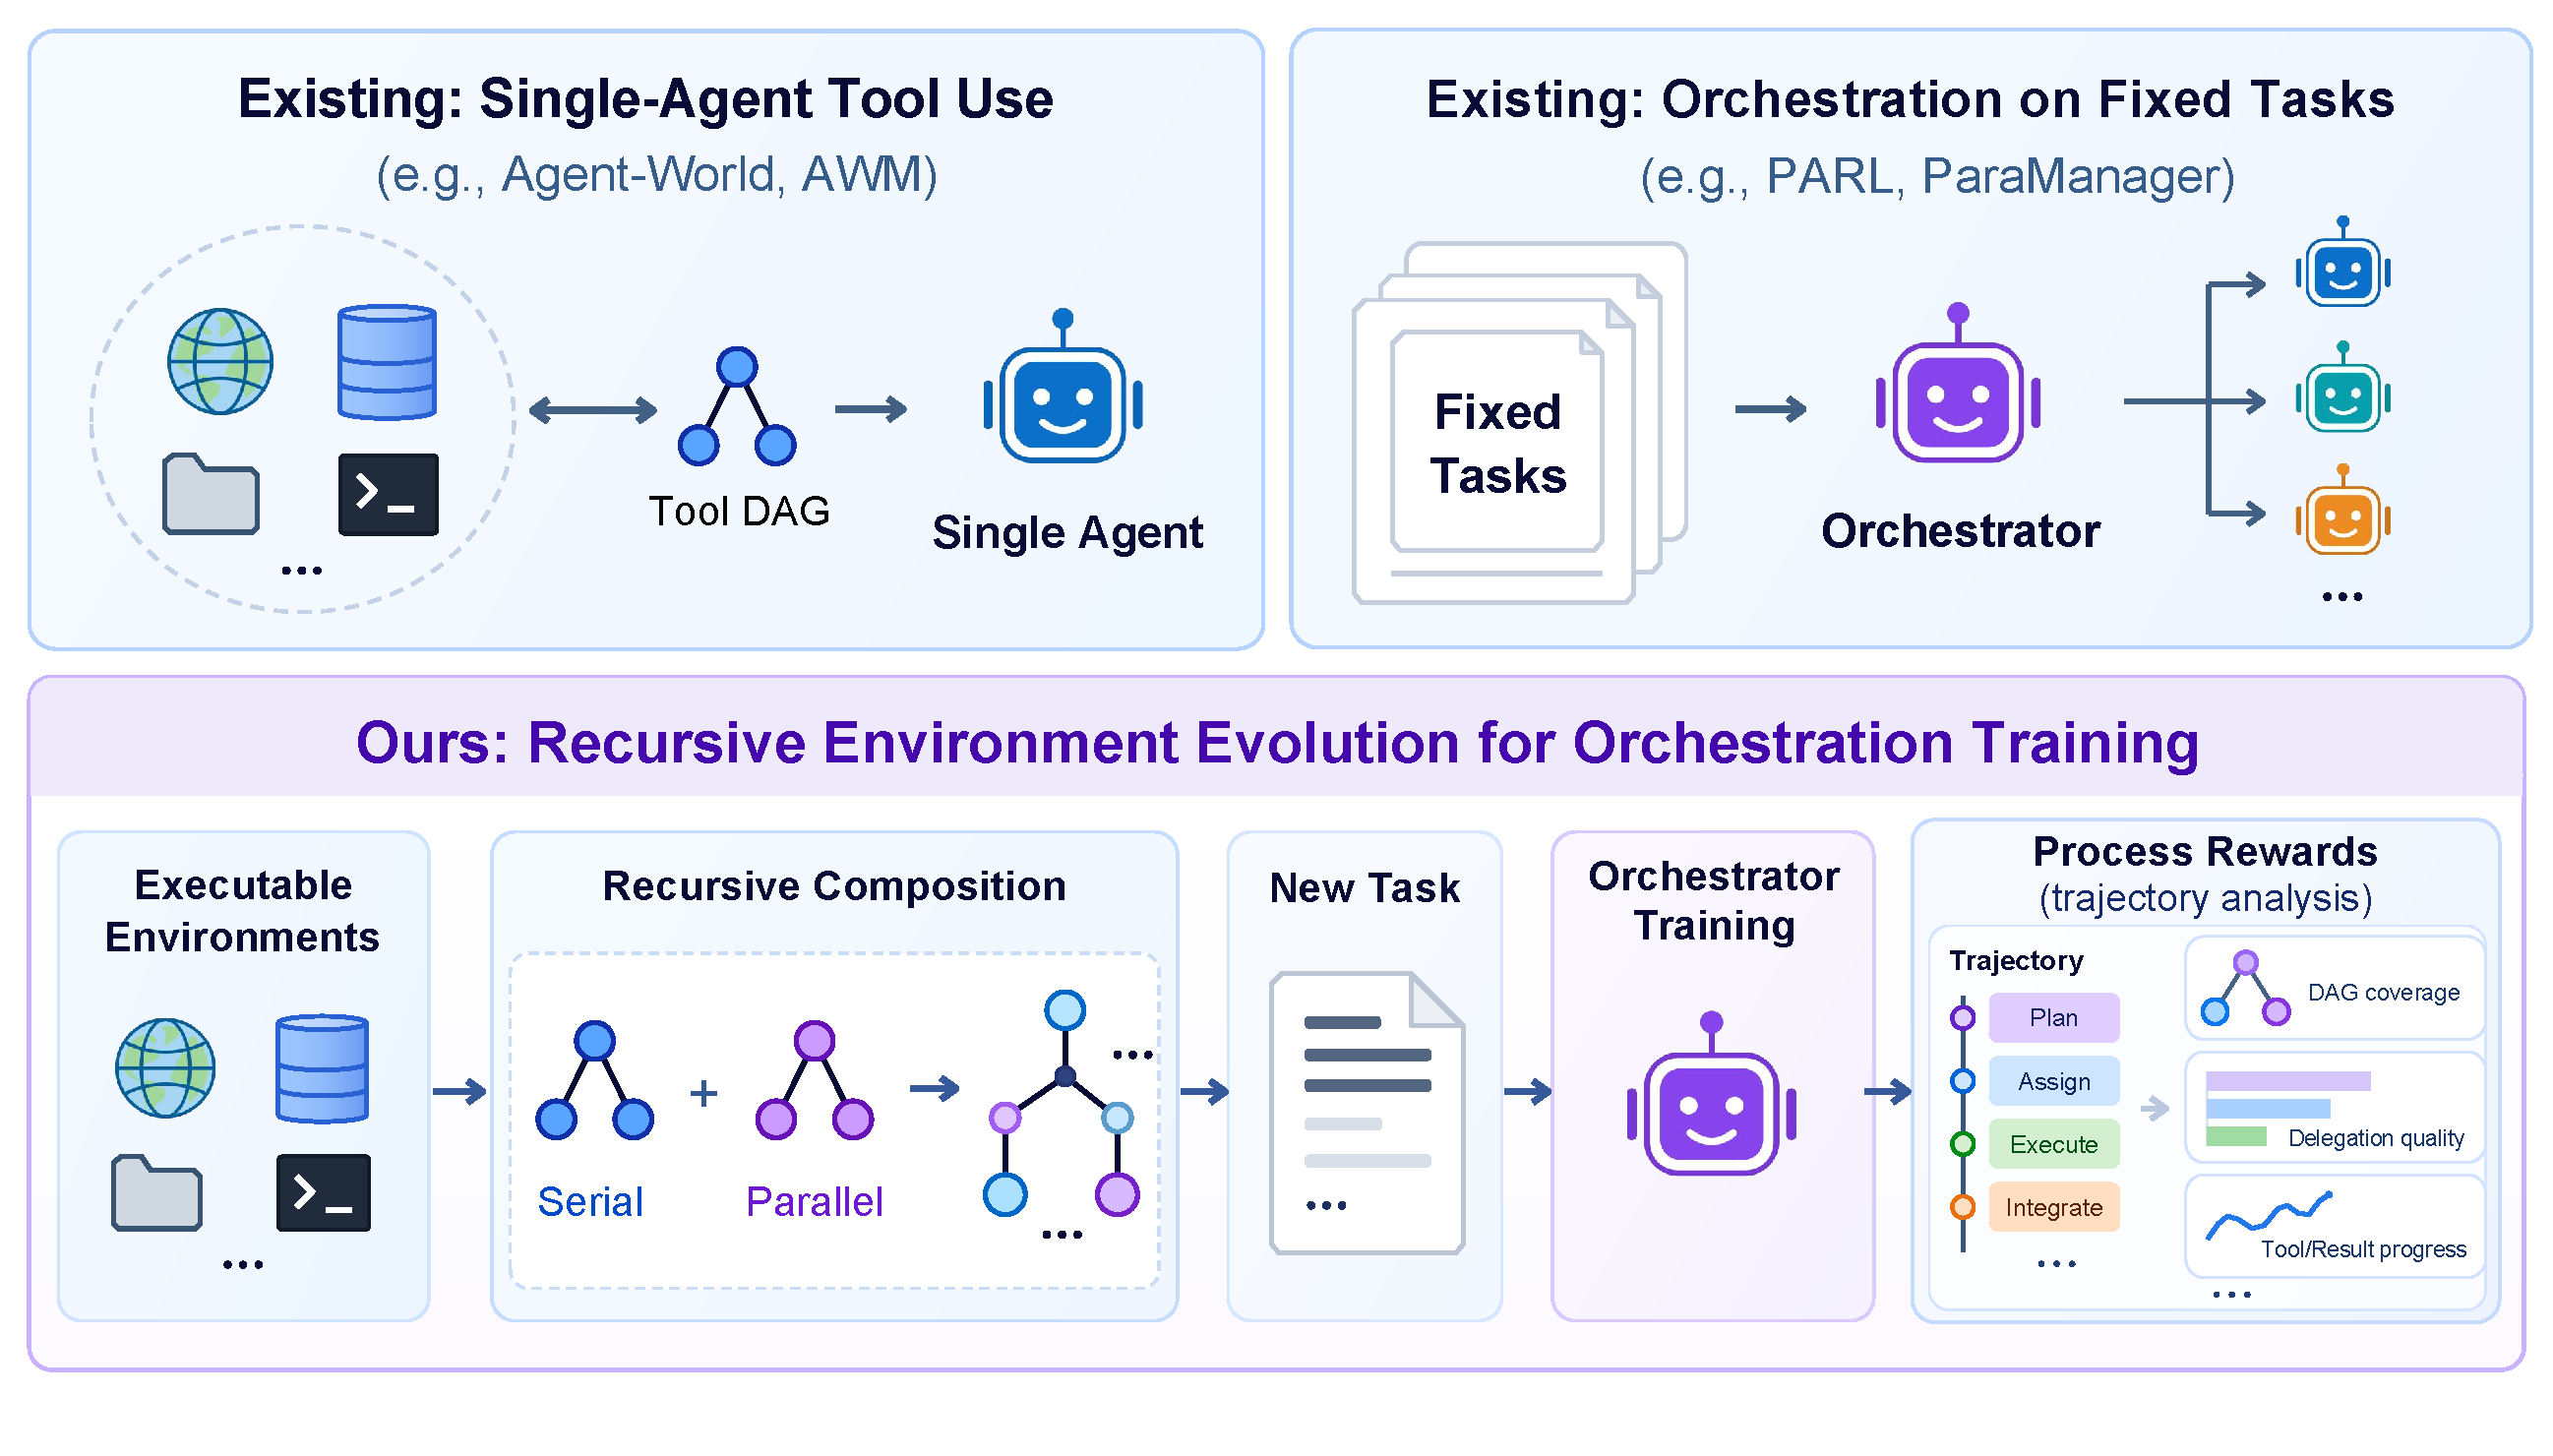
\includegraphics[width=0.97\linewidth]{figures/figure1.pdf}
  \caption{Existing environment synthesis builds executable tools and a verifier for one agent, and existing orchestration training consumes a fixed task set whose branch structure it does not control. MAW evolves the tasks of an executable environment by recursive environment improvement and trains an orchestrator on the resulting branches under schedule-aware process rewards.}
  \label{fig:teaser}
\end{figure}

To this end, we introduce \emph{Multi-Agent World} (MAW), an end-to-end framework for developing multi-agent orchestration.
As shown in Figure~\ref{fig:teaser}, MAW couples multi-agent environment synthesis with reinforcement learning inside the synthesized environments.
Specifically, to close the structural gap, MAW synthesizes multi-agent environments by \emph{recursive environment improvement}.
A serial operator links a subtask to the effect it consumes, and a parallel operator places independent subtasks on separate branches.
Applying the two operators recursively grows a reference task graph, which semantic reconstruction then rewrites into one coherent user request.
After the reference executes, replays from a fresh state, and passes semantic review, MAW admits the task into the training set.
To close the supervision gap, MAW trains the orchestrator with \emph{schedule-aware process rewards}.
These rewards read the recorded execution of the whole team and score tool progress, answer coverage, evidence delivery, and the quality of the schedule itself.
MAW connects the two mechanisms through one record.
Composition writes the branch structure into a task, and in the same step records which subtasks are verified as independent.
This record distinguishes a correct parallel decomposition from one that succeeds by chance.
Multi-agent environment synthesis therefore produces both the environment in which the team acts and the ground truth against which the orchestrator is rewarded.

We evaluate MAW on six agentic benchmarks covering multi-turn tool use, interactive task completion, executable multi-step tasks, long-horizon planning, broad information seeking, and real-world tool execution.
Experimental results show that MAW improves task success by \fillin\ over its single-agent initialization and by \fillin\ over the same multi-agent runtime without an orchestration update, while shortening the execution critical path by \fillin.
More importantly, the ablations show that the branches introduced by composition, and not the additional length of a composed task, account for the improvement.
Our contributions are three-fold.
\begin{itemize}[leftmargin=1em, itemsep=-1ex, topsep=0ex]
  \item \textbf{End-to-End Multi-Agent Framework}: To the best of our knowledge, MAW is the first framework that develops multi-agent orchestration end to end, synthesizing multi-agent environments and training the orchestrator inside them, where the construction record of a task also serves as the ground truth of its reward.
  \item \textbf{Recursive Environment Improvement and Schedule-Aware Rewards}: We propose recursive environment improvement, which converts single-agent environments into multi-agent environments by treating branch structure as a controlled construction variable, and schedule-aware process rewards, which make the quality of a decomposition visible in the gradient before any complete solution is sampled.
  \item \textbf{Strong Performance}: Experimental results on six agentic benchmarks show that MAW improves task success by \fillin\ with an 8B backbone, and behavior audits show that the gain comes from fewer duplicated assignments and fewer missing integrations.
\end{itemize}

\section{Related Work}
\label{sec:rw}

\paragraph{Environment Synthesis for Single-Agent Training.}
Training an agent with reinforcement learning requires environments that execute, hold state, and verify outcomes automatically, and a recent line of work builds such environments at scale for one agent.
AWM synthesizes code-backed worlds with structured databases and rule-based checkers, thereby delivering a task with executable tools and a verifiable answer~\citep{wang2026agentworldmodelinfinity}.
EnvScaler separates the construction of an environment skeleton from the generation of scenarios and validators, which raises the yield of usable tasks~\citep{song2026envscaler}.
Agent-World pairs environment discovery with a diagnostic loop that keeps tasks near the current ability of the policy~\citep{dong2026agentworld}, and ToolVerse follows tool dependencies to build long-horizon tasks~\citep{zhou2026toolverse}.
Further work adapts existing environments through interface components or learns an environment-design role through self-play~\citep{huang2026envharness,liu2026spade}.
Overall, these systems produce executable and automatically verified tasks for a single agent that observes every tool return itself.
Such a task rarely contains subtasks that several agents can execute simultaneously, and its verifier reports only whether one agent finished.

\paragraph{Multi-Agent Collaboration and Orchestration Training.}
Multi-agent systems differ mainly in how the collaboration structure is decided.
AutoGen organizes collaboration as conversations between agents~\citep{wu2023autogenenablingnextgenllm}, and MetaGPT encodes standardized operating procedures as role-based workflows~\citep{hong2024metagptmetaprogrammingmultiagent}.
In both cases a human authors the structure and the structure stays fixed during execution.
A second group searches the structure automatically, through optimizable agent graphs~\citep{zhuge2024languageagentsoptimizablegraphs}, workflow generation~\citep{zhang2025aflowautomatingagenticworkflow,hu2025automateddesignagenticsystems}, and agentic supernets that select a topology per query~\citep{zhang2025maasagenticsupernet}.
Although search improves the structure, the selected structure still fixes collaboration once execution starts.
A third group updates the model that performs the orchestration.
Representative methods include evolving orchestration for agent collaboration~\citep{dang2025puppeteer}, parallel agent reinforcement learning that credits critical steps~\citep{kimiteam2026kimik25}, and unified agent and tool orchestration with parallel subtask decomposition~\citep{yuan2026paramanager}.
Overall, learned orchestration is established as feasible.
In these studies, the branch structure of the training distribution is inherited from existing benchmarks, thereby remaining neither controlled during construction nor available during reward computation.

\paragraph{Positioning of MAW in Multi-Agent Training.}
In this work, we focus on how the multi-agent environments an orchestrator trains in relate to the signal it trains under.
Within backends that already execute and verify, our goal is to scale orchestration training.
Unlike environment synthesis that targets a single agent, MAW treats branch structure as a construction variable and composes reference task graphs with serial and parallel operators.
Dependencies and independent branches are thereby written into a task on purpose.
Unlike orchestration learning that consumes a fixed task distribution and scores a rollout by terminal success, MAW adopts a more deliberate design by carrying the construction record into training.
Specifically, the schedule of the agent team is scored against the independent subtasks that composition has already verified.
We state what is new here precisely.
Learned orchestration and synthesized environments have both been studied, and synthesizing an environment for the orchestration signal itself has not.
In MAW, one construction supplies the task, its branches, and the ground truth that scores how those branches are used.

\section{Multi-Agent World}
\label{sec:method}

As shown in Figure~\ref{fig:overview}, MAW develops multi-agent orchestration in two stages that share one construction record.
The first stage turns existing single-agent backends into multi-agent environments, in which a task carries subtasks that several agents can execute simultaneously.
The second stage trains an orchestrator inside those environments under a reward that reads how the agent team actually distributed the work.


\begin{figure}[t]
  \centering
  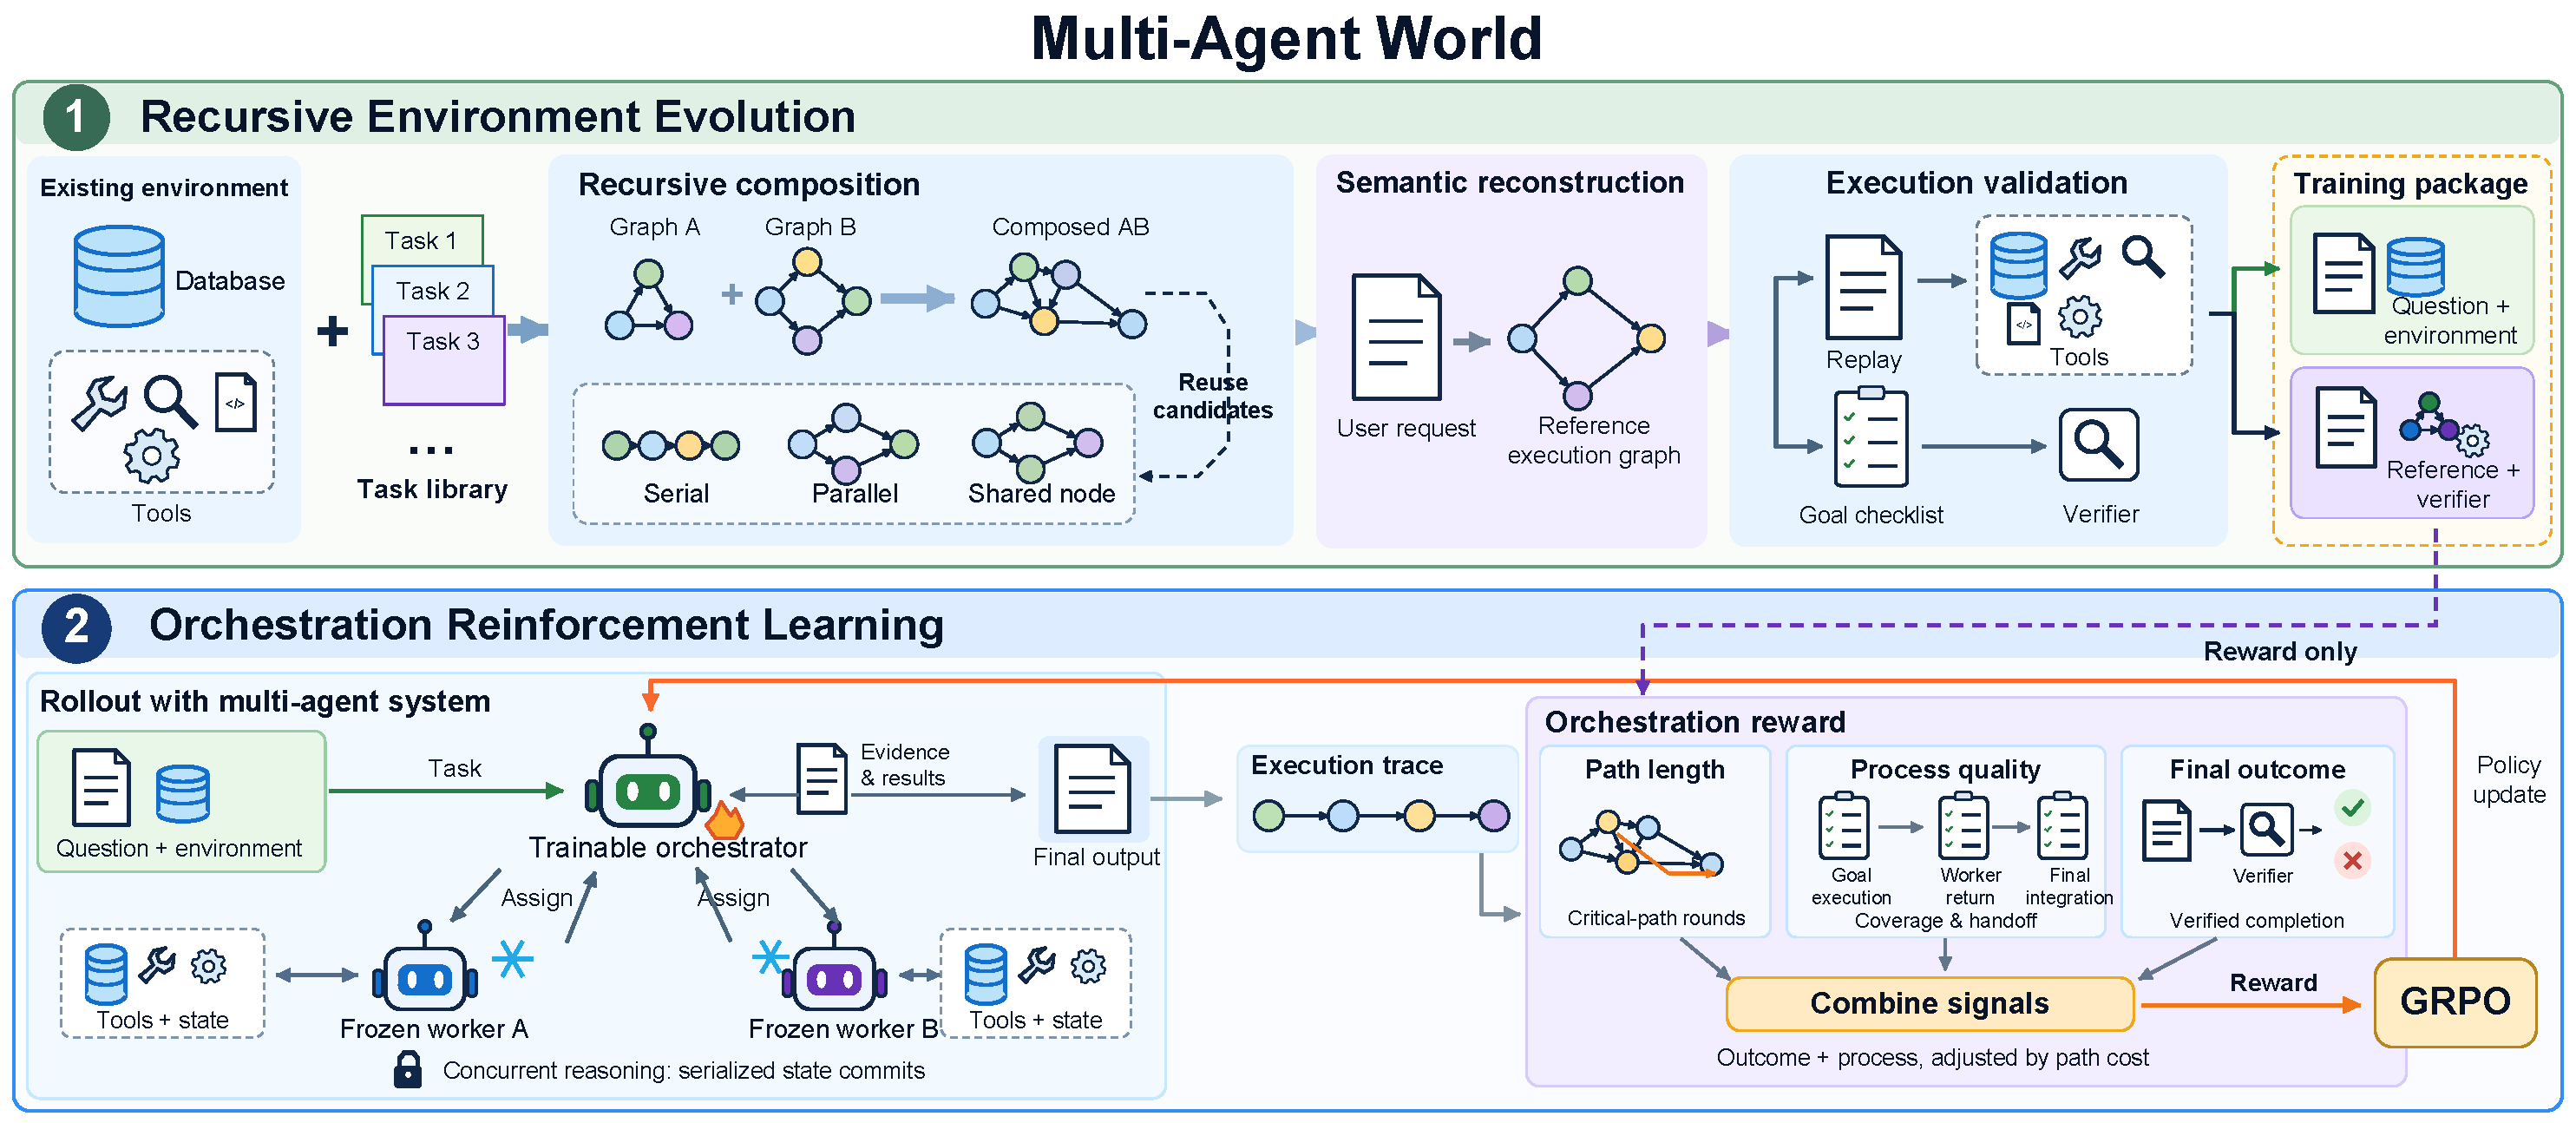
\includegraphics[width=0.99\linewidth]{figures/figure2.pdf}
  \caption{Overview of MAW. Recursive environment improvement composes the reference graphs of existing tasks, reconstructs each composed graph into one request, and admits it only after replay and verification. The resulting package supplies the interactive environment to the agent team and the hidden reference to the reward service, and only the orchestrator is updated.}
  \label{fig:overview}
\end{figure}

\subsection{From Single-Agent to Multi-Agent Environments}
\label{sec:ma-env}

An agentic environment is written as $\mathcal{E}=(\mathcal{S},\mathcal{U},f_{\mathrm{exec}},s_0)$, where $\mathcal{S}$ is a database-backed state space, $\mathcal{U}$ is the tool interface, and $s_0$ is the initial state.
The transition $f_{\mathrm{exec}}(s,u)=(s',o)$ executes a tool call $u$ and returns an observation $o$.
Following the synthesis setting of AWM and Agent-World~\citep{wang2026agentworldmodelinfinity,dong2026agentworld}, a task in $\mathcal{E}$ is written as $x=(q,G,a^{\star},\Delta^{\star})$.
Here $q$ is the user request, $a^{\star}$ is the reference answer, and $\Delta^{\star}$ is the required change of the database.
The reference task graph $G=(V,A)$ has one node $v\in V$ per reference tool call, and an edge $(u,v)\in A$ means that $v$ consumes an output or a state effect of $u$.

A multi-agent environment extends this setting with a delegation interface and an independence record.
The interface $\mathcal{H}$ lets an orchestrator create workers and assign subtasks to them, which is what makes a team executable at all.
The record $\Pi$ closes the supervision gap of Section~\ref{sec:intro}, since it names the branches against which a schedule can be scored, while the structural gap is closed by the composition that creates those branches.
We write a multi-agent environment as $\mathcal{E}^{\mathrm{ma}}=(\mathcal{S},\mathcal{U},f_{\mathrm{exec}},s_0,\mathcal{H})$ and a multi-agent task as $x^{\mathrm{ma}}=(q,G,a^{\star},\Delta^{\star},\Pi)$.
Here $\Pi\subseteq V\times V$ contains the pairs of reference calls that are verified to be executable in either order.
Orchestration training consumes this record, without which a verifier reports only whether the team produced the correct answer and leaves the correctness of a simultaneous execution unmeasured.
Existing pipelines produce $(q,G,a^{\star},\Delta^{\star})$ for one agent and leave $\Pi$ empty, which is why their tasks train tool use and not orchestration.

\subsection{Recursive Environment Improvement}
\label{sec:synthesis}

In this stage, we aim to turn existing single-agent backends into multi-agent environments without building new ones from scratch, which is challenging as branch structure cannot be requested from a generator directly.
When a model is asked for a parallel task, it tends to produce two unrelated questions in one prompt, leaving an executable reference that is either trivial or inconsistent.
MAW instead constructs branch structure at the level of reference graphs, where independence is a checkable property, and writes the graph as natural language only afterwards.

\textbf{Recursive Composition.}\quad
Before any natural language is generated, composition introduces a controlled amount of dependency and independence into a task.
From a seed pool $\mathcal{C}$ of single-agent tasks in the same backend, MAW composes two of them into a candidate graph,
\begin{equation}
\tilde{G}=f_{\mathrm{comp}}^{z}(G_1,G_2),\qquad z\in\{\mathrm{serial},\mathrm{parallel}\},
\label{eq:compose}
\end{equation}
where the serial operator adds an edge between a pair $(v_1,v_2)\in V_1\times V_2$ whose output or state effect fills an argument of the other.
In contrast, the parallel operator takes the disjoint union with no edge between the two sides and lets one answer node consume both.
After composition, a candidate graph re-enters $\mathcal{C}$ and acquires further subtasks in later rounds, so mixed structure arises from repeated application.
For each edge, MAW stores the operator that produced it, which later distinguishes a branch from an accidental ordering, and Appendix~\ref{app:synthesis} gives a worked example of two rounds.


\textbf{Semantic Reconstruction.}\quad
A composed graph is not yet a request a user would write, as the two parents may refer to different entities or reporting formats.
Reconstruction produces one coherent request and an executable reference plan, written as $(q,G)=f_{\mathrm{recon}}(\tilde{G},q_1,q_2,\mathcal{U})$, during which MAW aligns entities across the two sides, merges reads that return the same content, and inserts a lookup when the combined goal needs one.
The request states the desired outcome and exposes neither the reference plan nor any hint about how many workers to use, thereby leaving the decomposition to the policy.

\textbf{Execution-grounded Admission.}\quad
As repeated composition can accumulate redundant calls or combine requirements that no single execution satisfies, MAW admits a task only when its reference survives execution and inspection.
Executing the plan from a reset state gives $(a^{\star},\Delta^{\star})=f_{\mathrm{exec}}^{\ast}(G,s_0)$, and MAW then replays it from a fresh state.
MAW admits a task only when execution, replay, and an independent review all pass, written as $f_{\mathrm{gate}}=f_{\mathrm{run}}\cdot f_{\mathrm{replay}}\cdot f_{\mathrm{sem}}\in\{0,1\}$ and specified in Appendix~\ref{app:synthesis}.
Admission is the step that keeps a composed candidate from entering training as an unsolvable or self-contradictory task.

\textbf{Verified Independence Record.}\quad
Although composition proposes that two subtasks lie on separate branches, the proposal is not yet verified, as reconstruction may introduce a shared entity that makes one side depend on the other.
MAW verifies every proposed branch by execution before recording it,
\begin{equation}
\Pi=\bigl\{(v,v')\in V_{\mathrm{r}}\times V_{\mathrm{r}} \,:\, v\nprec v',\; v'\nprec v,\; f_{\mathrm{perm}}(v,v')=1\bigr\},
\label{eq:pi}
\end{equation}
where $V_{\mathrm{r}}\subseteq V$ is the set of read-only calls and $v\prec v'$ denotes that $v'$ is reachable from $v$ in $G$.
The test $f_{\mathrm{perm}}(v,v')$ executes the reference plan again with the order of the two calls exchanged, returning one when the answer and the database effect are unchanged.
Together with its resettable environment, its checker, and its hidden reference, this record converts a synthesized task into a multi-agent task.
One construction therefore produces two things at once, namely the branches an orchestrator can act on and the ground truth against which its use of those branches is scored.
Section~\ref{sec:learning} consumes the second of them.

\subsection{Multi-Agent Orchestration Learning with Schedule-aware Process Rewards}
\label{sec:learning}

In this stage, we aim to teach an orchestrator to distribute work well, which terminal verification alone cannot express, as it collapses every unfinished team execution into the same value.
A group of rollouts that all fail produces identical returns, and their centered advantages vanish.
The task then contributes no gradient during the stage where the policy fails most often.
MAW addresses this by reading the recorded execution of the whole team and scoring the part of the work that was done correctly, including the schedule itself.

\textbf{Delegation-only Interaction Harness.}\quad
In the MAW harness, delegation is the only way to act, attributing every reward difference to orchestration and not to the orchestrator solving the task directly.
Specifically, the orchestrator $\pi_\theta$ registers a worker with a role and a permitted tool subset through \texttt{create\_subagent}.
The orchestrator then assigns one subtask through \texttt{assign\_task}, assigns several subtasks concurrently through \texttt{assign\_tasks}, and ends the episode through \texttt{submit\_answer}.
During an episode, every worker follows the frozen policy $\pi_\phi$ and is the only actor that accesses $\mathcal{U}$.
The runtime records each tool event with its arguments, observation, owning assignment, and causal parents, which is the record the reward reads, and Appendix~\ref{app:runtime} states the information boundary between the three participants.

\textbf{Team-Level Outcome Verification.}\quad
In a multi-agent setting, the outcome term determines whether the team completed the task by verifying the environment and not the report of any agent.
For a trajectory $\tau$ with final answer $a_\tau$ and final state $s_\tau$, the outcome term requires both an accepted answer and an accepted database state,
\begin{equation}
f_{\mathrm{out}}(\tau)=V^{\mathrm{ans}}\bigl(a_\tau,a^{\star}\bigr)\cdot V^{\mathrm{state}}\bigl(\Delta_\tau,\Delta^{\star}\bigr)\in\{0,1\},
\label{eq:outcome}
\end{equation}
where $V^{\mathrm{ans}}$ and $V^{\mathrm{state}}$ are the answer and state checkers of the task, each returning one when the submitted result is accepted and zero when an episode ends without a submission.
The state checker compares the required database mutations and rejects unexpected changes.
Receiving only the account of a worker, the orchestrator can do no more than repeat it, so checking $\Delta_\tau$ is what establishes that a record was created or updated and that unrelated rows were left untouched.


\begin{figure}[t]
  \centering
  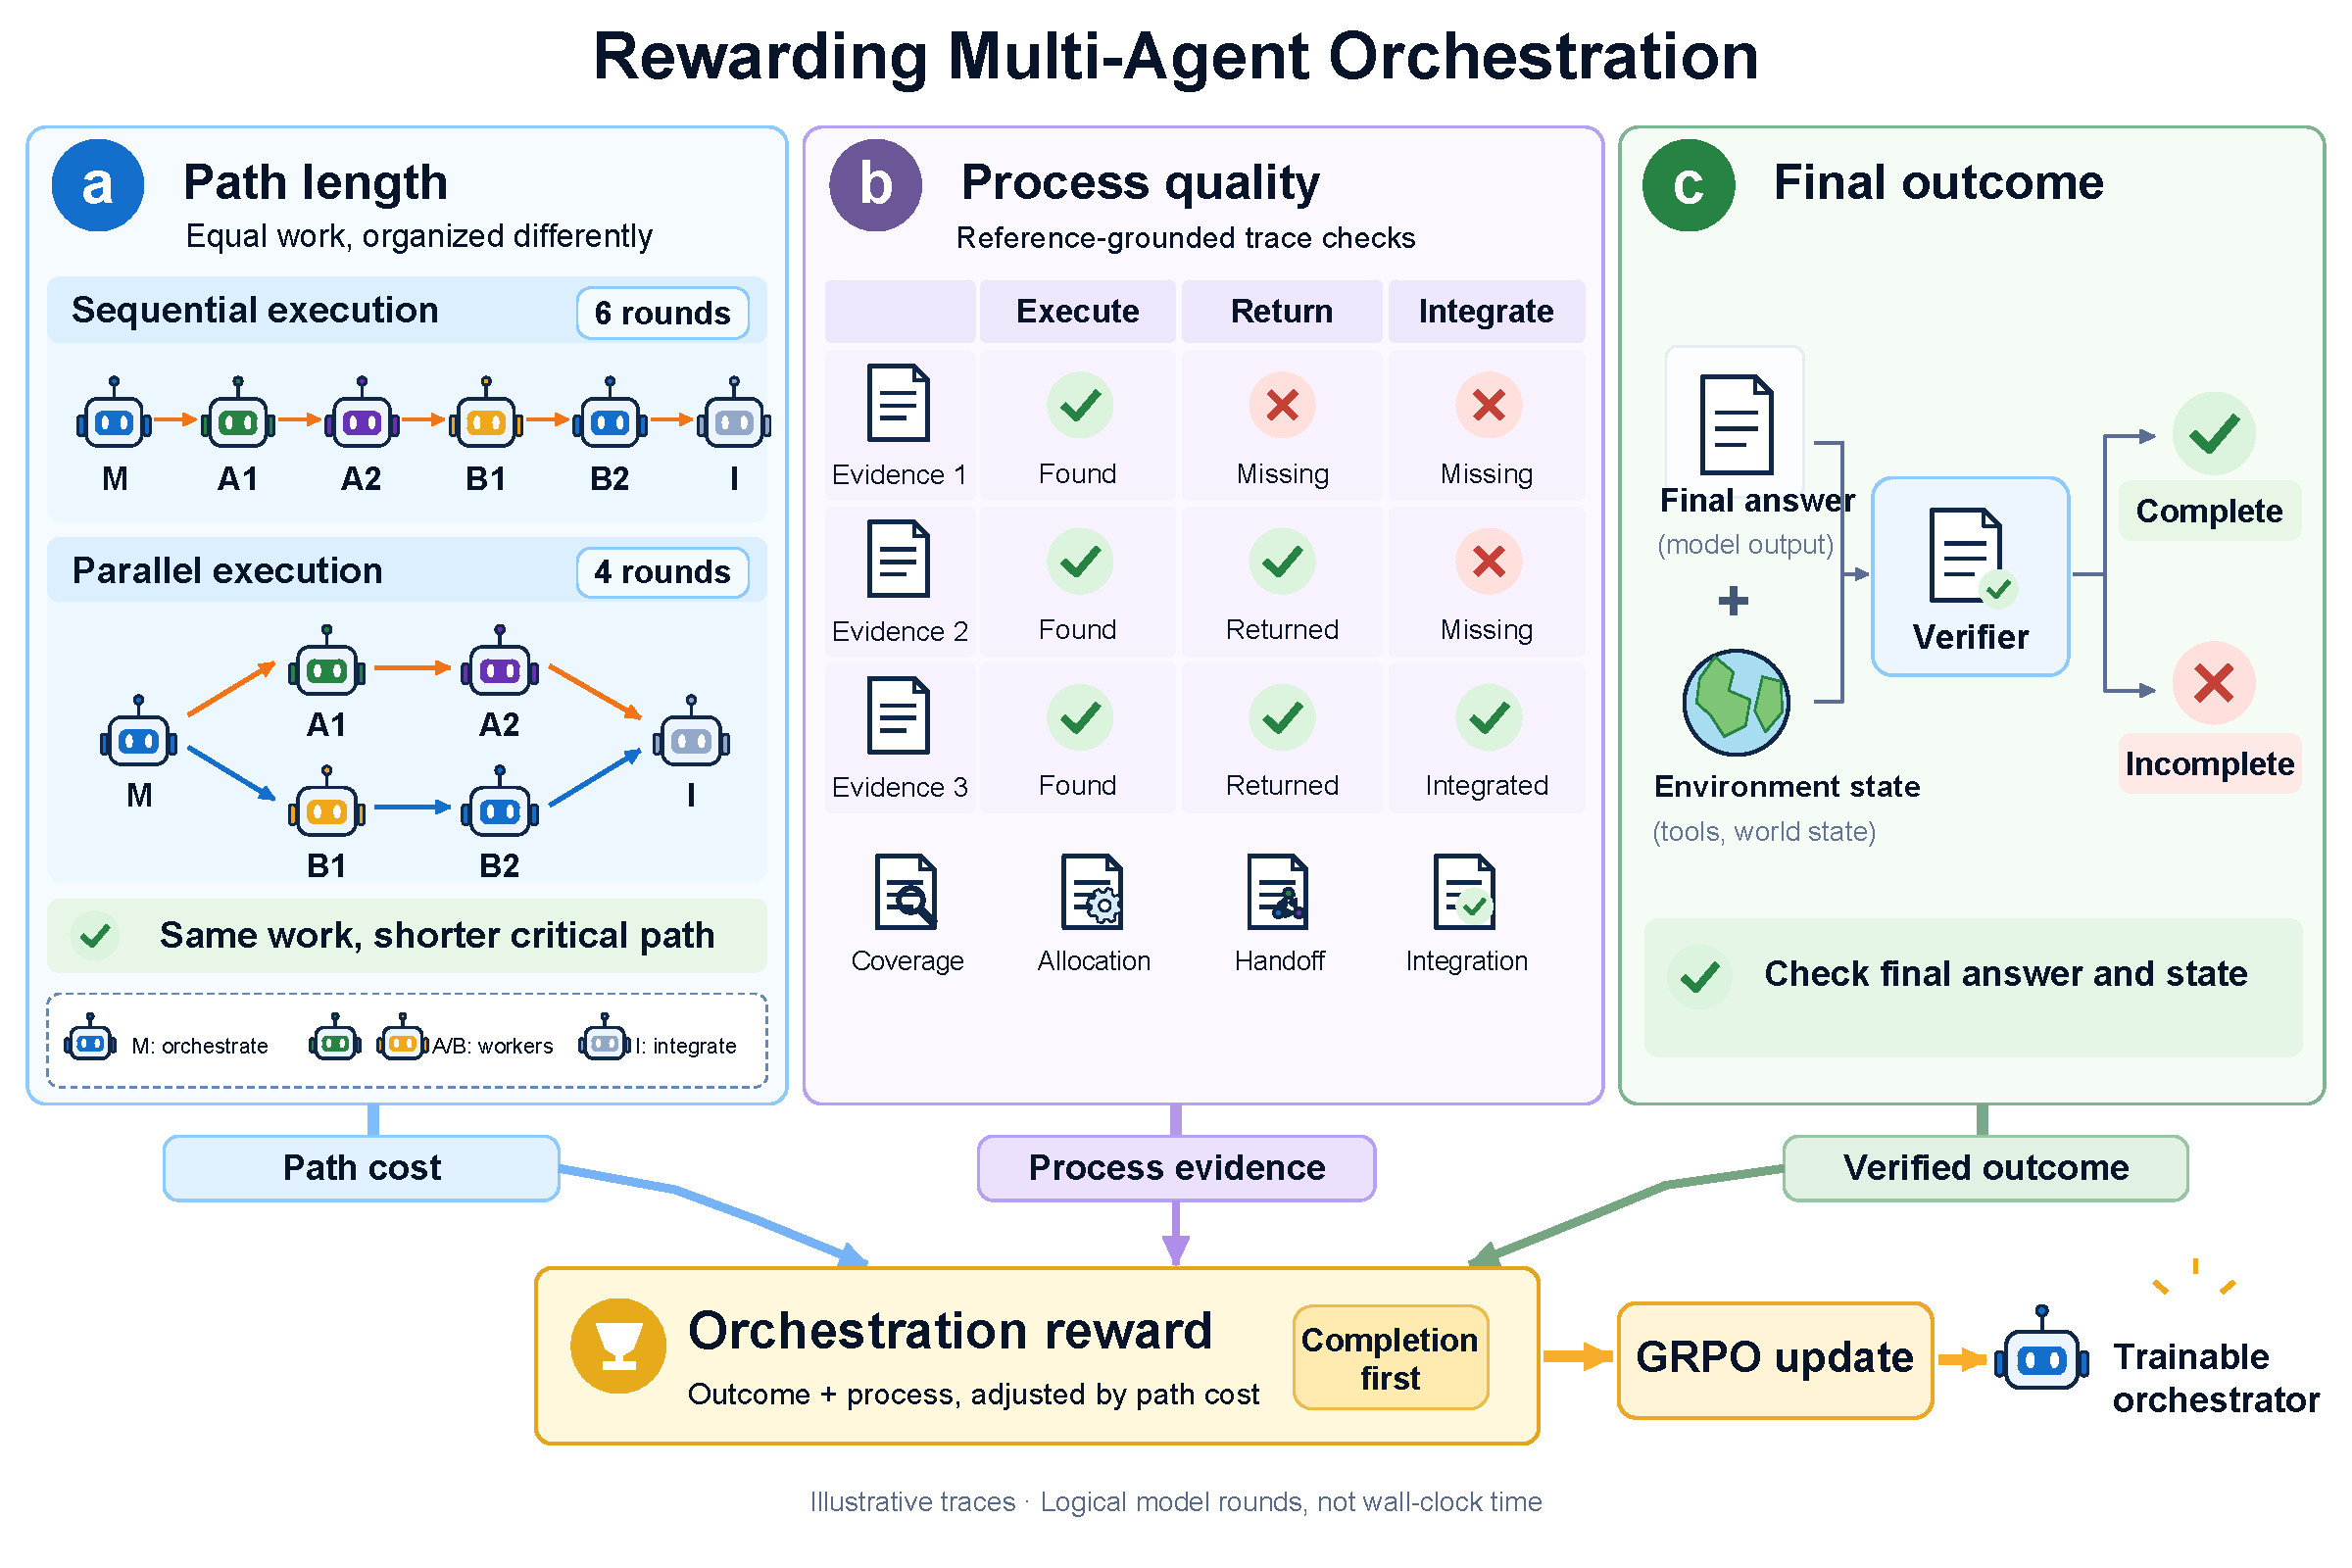
\includegraphics[width=\linewidth]{figures/figure4.pdf}
  \caption{Three sources of the orchestration reward. Equal work organized in parallel shortens the critical path (a), reference-grounded checks separate execution, return, and integration for every piece of evidence (b), and the verifier accepts a trajectory only when the final answer and the environment state both hold (c).}
  \label{fig:reward}
\end{figure}

\textbf{Schedule-aware Process Reward.}\quad
As shown in Figure~\ref{fig:reward}, the process term scores four properties of a team execution, namely the reference work completed, the requested answer present, the evidence returned by workers, and the independent work scheduled as independent,
\begin{equation}
f_{\mathrm{proc}}(\tau)=\alpha_{\mathrm{t}}f_{\mathrm{tool}}(\tau)+\alpha_{\mathrm{a}}f_{\mathrm{ans}}(\tau)+\alpha_{\mathrm{d}}f_{\mathrm{del}}(\tau)+\alpha_{\mathrm{s}}f_{\mathrm{sch}}(\tau),
\label{eq:proc}
\end{equation}
where every term lies in $[0,1]$ and the weights $\alpha$ are fixed once for all experiments (Table~\ref{tab:config}).
The tool term $f_{\mathrm{tool}}$ is the fraction of reference calls in $V$ matched once by a successful event with equivalent arguments and observation.
The answer term $f_{\mathrm{ans}}$ gives recall-oriented partial credit over the top-level fields of the answer, with a precision factor that removes any gain from padding the submission (Appendix~\ref{app:process}).
A team recovering most of the answer is thereby separated from one recovering none.
The delivery term $f_{\mathrm{del}}$ is the fraction of assigned subtasks whose worker return carries the required evidence, which measures the handoff a single agent never performs.
The schedule term is the part of the reward that no terminal verifier can express, and it reads the independence record produced by Eq.~\ref{eq:pi},
\begin{equation}
f_{\mathrm{sch}}(\tau)=(1-\delta_\tau)\cdot f_{\mathrm{int}}(\tau)\cdot\frac{|\Pi_\tau|}{|\Pi|},
\label{eq:sched}
\end{equation}
The leading ratio is the fraction of verified independent pairs that the team actually ran as independent, where $\Pi_\tau\subseteq\Pi$ contains the pairs assigned to two different workers under assignment intervals that do not depend on each other.
Two factors keep that ratio honest, since $\delta_\tau$ discounts assignments that repeat a covered subtask and $f_{\mathrm{int}}$ discounts branch results that never reach the final answer.
Eq.~\ref{eq:sched} is where synthesis and learning meet, as $\Pi$ exists only because composition proposed a branch and a reordered execution confirmed it.
A team is therefore credited for parallel work only on branches the environment has proven parallel, which is a judgement that terminal success cannot make.
A task whose reference contains no verified independent pair falls back to a conservative progress score, and Appendix~\ref{app:process} specifies that branch.

\textbf{Orchestrator-only Policy Optimization.}\quad
Partial progress requires enough weight to distinguish failing rollouts and little enough to never compete with a verified success.
The two terms are combined as
\begin{equation}
R(\tau)=f_{\mathrm{out}}(\tau)+\lambda\,f_{\mathrm{proc}}(\tau),\qquad \lambda=0.3,
\label{eq:reward}
\end{equation}
which gives a successful team at least $1$ and an unsuccessful team at most $\lambda$.
Process credit thereby separates failed rollouts without ever outweighing success.
For each task we sample $K$ team trajectories from independently reset environments and compute the group-relative advantage $A_i=(R_i-\bar{R})/(\mathrm{std}(R_1,\dots,R_K)+\epsilon)$ of the $i$-th trajectory.
The orchestrator is then updated with the clipped GRPO objective~\citep{shao2024deepseekmath}, written as
\begin{equation}
J(\theta)=\mathbb{E}\Bigl[\tfrac{1}{K}\textstyle\sum_{i=1}^{K}\tfrac{1}{|\mathcal{T}_i|}\sum_{t\in\mathcal{T}_i}\min\bigl(\rho_{it}(\theta)A_i,\ \mathrm{clip}(\rho_{it}(\theta),1-\epsilon_l,1+\epsilon_h)A_i\bigr)\Bigr],
\label{eq:grpo}
\end{equation}
where $\mathcal{T}_i$ contains only the tokens generated by the orchestrator and $\rho_{it}$ is the ratio between the current and the behavior policy on that token.
Worker generations and tool observations enter the context of the orchestrator and stay out of $\mathcal{T}_i$.
Since $\pi_\phi$ is never updated, every measured change comes from orchestration and not from worker quality.

\section{Experiments}
\label{sec:exp}

\subsection{Benchmarks}

We evaluate on six agentic benchmarks that together cover the decisions an orchestrator makes.
\textbf{BFCL Multi-Turn}~\citep{patil2025bfcl}, \textbf{$\tau^2$-Bench}~\citep{barres2025tau2bench}, and \textbf{ACEBench-Agent}~\citep{chen2025acebench} measure tool use across turns, interactive completion under a simulated user, and executable multi-step tasks, and they are dominated by dependent call sequences.
In contrast, \textbf{DeepPlanning}~\citep{zhang2026deepplanning}, \textbf{WideSearch}~\citep{wong2025widesearch}, and \textbf{MCPMark}~\citep{wu2025mcpmark} measure long-horizon planning under verifiable constraints, broad information seeking that fills one structured table, and real tool execution through Model Context Protocol services, and their requests carry evidence that can be gathered along several branches.
Together, the two groups measure orchestration from complementary directions, and Appendix~\ref{app:training} records the evaluation protocol.

\subsection{Baselines}

Under one runtime and one budget, we compare MAW with four groups of systems.
\emph{Frontier models} run as single agents under the same tool access and indicate the headroom of each benchmark, and \emph{open-source backbones} are the untrained Qwen3-8B and Qwen3-14B models~\citep{yang2025qwen3}, of which Qwen3-8B initializes every trained system.
\emph{Single-agent environment synthesis} covers AWM~\citep{wang2026agentworldmodelinfinity}, EnvScaler~\citep{song2026envscaler}, and ToolVerse~\citep{zhou2026toolverse}.
Each trains the same backbone on its released resources under a common outcome-based recipe, testing the utility of a training resource without reproducing every optimization detail of the original system.
\emph{Orchestration training} covers Puppeteer~\citep{dang2025puppeteer} and ParaManager~\citep{yuan2026paramanager}, together with two settings of our own system.
\emph{Single-agent (init)} is the trained single-agent checkpoint that initializes MAW, executed without workers, and it is the reference point for every gain we report.
\emph{Multi-agent (init)} runs the MAW runtime with that same checkpoint as an orchestrator and applies no orchestration update, which isolates the effect of the execution architecture alone.

\subsection{Setup}

We build MAW on Qwen3-8B and initialize the orchestrator and the workers from the same single-agent checkpoint, thereby attributing any measured difference to orchestration training.
Multi-agent environment synthesis runs over publicly released tool backends and admits 2,581 tasks across 539 environments, which we use for orchestration training.
In every comparison, the generator and the semantic reviewer use the same frontier model.
With the worker policy frozen, we train the orchestrator with GRPO under Eq.~\ref{eq:reward} and sample $K=8$ team trajectories per task from independently reset environments.
Inference uses the vLLM engine, and all training and evaluation run on NVIDIA A800 GPUs.
Every benchmark applies one shared token budget, timeout, worker-concurrency cap, and decoding configuration across compared systems, with failed and timed-out episodes kept in the denominator.

\begin{table}[t]
\centering
\small
\caption{Performance on six agentic benchmarks. Every trained system uses a Qwen3-8B backbone, and Qwen3-14B is listed as an untrained reference only. Metrics are multi-turn accuracy, task success, case accuracy, item F1, and pass rate, all in \%. \colorbox{gray!15}{Shaded} marks our method and \textbf{bold} marks the best 8B result per column.}
\label{tab:main}
\setlength{\tabcolsep}{5pt}
\renewcommand{\arraystretch}{1.12}
\begin{tabular}{@{}lcccccc@{}}
\toprule
\multirow{2}{*}{Model} & BFCL MT & $\tau^2$-Bench & ACEBench & DeepPlanning & WideSearch & MCPMark \\
 & Accuracy & Success & Success & Case Acc. & Item F1 & Pass Rate \\
\midrule
\multicolumn{7}{@{}l}{\textit{Frontier Models}} \\
DeepSeek-V3.2 & 37.39 & 80.37 & 80.62 & & & \\
GPT-4.1 & 38.88 & 54.67 & 82.92 & & & \\
Kimi-K2-Instruct & 50.63 & 64.30 & 79.17 & & & \\
\midrule
\multicolumn{7}{@{}l}{\textit{Open-Source Backbones}} \\
Qwen3-14B & & & & & & \\
Qwen3-8B & 28.88 & 27.87 & 46.51 & & & \\
\midrule
\multicolumn{7}{@{}l}{\textit{Single-Agent Environment Synthesis}} \\
AWM & & & & & & \\
EnvScaler & & & & & & \\
ToolVerse & 37.50 & 32.37 & 61.66 & & & \\
\midrule
\multicolumn{7}{@{}l}{\textit{Orchestration Training (8B)}} \\
Single-agent (init) & & & & & & \\
Puppeteer & & & & & & \\
ParaManager & & & & & & \\
Multi-agent (init) & & & & & & \\
\rowcolor{gray!15}
MAW (ours) & & & & & & \\
\bottomrule
\end{tabular}
\end{table}


\subsection{Main Results}

\textbf{Capability on Dependent Tool Use.}\quad
We first evaluate MAW on BFCL Multi-Turn, $\tau^2$-Bench, and ACEBench-Agent to assess its \emph{dependent tool-use capability}.
In this group, a request expands into a chain of calls that leaves little to schedule, where each call depends on the effect of the earlier ones.
As shown in Table~\ref{tab:main}, MAW reaches \fillin\ on BFCL Multi-Turn and \fillin\ on $\tau^2$-Bench, exceeding every 8B system in the comparison.
On ACEBench-Agent it stays within \fillin\ of the strongest single-agent synthesis baseline.
Across the three benchmarks, MAW gains most on settings where a team can verify before committing, as a withheld function or a user-modified record is recovered by assigning a verification subtask.
However, multi-agent (init) loses accuracy on the same settings, which stems from assignments that no worker can satisfy.
Overall, the results on this group show that MAW improves the tool use a single agent already performs, without degrading the dependent call chains of the backbone.

\textbf{Capability on Branch-rich Long-horizon Tasks.}\quad
We then evaluate MAW on DeepPlanning, WideSearch, and MCPMark to assess its \emph{capability on separable work}.
In this group, constraint checks, retrievals, and service calls proceed along several branches before they are combined.
As shown in Table~\ref{tab:main}, MAW raises case accuracy by \fillin\ on DeepPlanning, reaches \fillin\ item F1 on WideSearch, and improves the MCPMark pass rate by \fillin.
Notably, multi-agent (init) falls below single-agent (init) on MCPMark, where an untrained orchestrator increases cost and does not improve success.
Recursive environment improvement produces the same kind of branch structure during synthesis, although over entirely different backends.
The orchestrator has thereby learned to assign independent checks to separate workers and to collect their results.
The audit in Section~\ref{sec:abl-reward} attributes the WideSearch improvement to fewer missing rows and not to more retrieval calls.
MAW also reaches these results at a shorter critical path than multi-agent (init), which Section~\ref{sec:abl-arch} reports alongside the token cost.
Overall, the strong results on this group highlight the transfer of synthesized branch structure to long-horizon tasks that the training distribution never contained.

\section{Analyses}
\label{sec:analysis}

\subsection{Ablation Study on Recursive Environment Improvement}
\label{sec:abl-construction}

To evaluate the effect of branch structure on the usefulness of a synthesized task, we compare six strategies for producing training tasks.
Across all rows, we keep the backends, the generator, the admission checks, and the outcome-only training recipe fixed.
The sources range from the original seeds and direct synthesis of a multi-goal request to one round of composition, recursion restricted to one operator, and full recursive environment improvement.
Measuring admitted tasks per generation budget alongside held-out success at an equal number of admitted tasks separates producing more usable data from producing more useful data.

\begin{table}[t]
\centering
\small
\caption{Ablation on multi-agent environment synthesis. All rows share the backends, the generator, the admission checks, and the outcome-only recipe. Yield is admitted tasks per fixed generation budget, $|\Pi|$ is the number of verified independent subtask pairs per admitted task, and success is held-out task success at an equal number of admitted tasks.}
\label{tab:abl-construction}
\setlength{\tabcolsep}{6pt}
\renewcommand{\arraystretch}{1.12}
\begin{tabular}{@{}lcccc@{}}
\toprule
Training-task source & Yield (\%) \up & Subtasks / task & $|\Pi|$ / task & Success (\%) \up \\
\midrule
Original seed tasks & & & & \\
Direct multi-goal synthesis & & & & \\
One-round composition & & & & \\
Recursive serial-only & & & & \\
Recursive parallel-only & & & & \\
\rowcolor{gray!15}
Recursive environment improvement (ours) & & & & \\
\bottomrule
\end{tabular}
\end{table}


As shown in Table~\ref{tab:abl-construction}, direct synthesis admits far fewer tasks than composition at the same budget.
This gap stems from writing two goals into one prompt before any execution, which frequently produces a reference that fails or contradicts itself.
In contrast, composition checks compatibility on reference graphs before any language is generated.
Under serial-only recursion, the admitted references are longer and carry almost no verified independent pairs.
Their held-out success also improves by less than that of full recursion, showing that task length alone does not train orchestration.
Under parallel-only recursion, the admitted tasks carry shallow dependencies and degrade on tasks that require waiting for a prerequisite.
Among the six sources, only full recursion admits tasks that carry a non-trivial $\Pi$ together with real dependencies, highlighting the effectiveness of applying the two operators recursively.
At the level of the distribution, reference tool calls grow by 19.6\% relative to the two parents of each task, while top-level answer fields grow by 57.3\% (Appendix~\ref{app:stats}).
A composed task thereby asks for more results that can be produced independently, which is the property an orchestrator can exploit.

\subsection{Ablation Study on Schedule-aware Process Rewards}
\label{sec:abl-reward}

To verify the effectiveness of each term of Eq.~\ref{eq:proc}, we conduct an ablation study that removes one term at a time, setting its coefficient to zero without redistributing the weight.
We also train an outcome-only setting.
All settings share the task set, the initialization, the frozen workers, the training budget, and the evaluation instances, thereby isolating the reward as the only difference.
The schedule term applies to the \fillin\ of training tasks that carry a verified independent pair, and the remaining tasks use the fallback score of Appendix~\ref{app:process}.
Besides task success, we audit held-out tasks whose reference annotations link every assignment to a subtask, reporting goal coverage, evidence delivery, duplicate allocation, handoff failure, and integration failure.
Together, these measurements distinguish a change in behavior from a change in score.

\begin{table}[t]
\centering
\small
\caption{Ablation on the schedule-aware process reward, with the behavior audit it targets. Each row sets one coefficient of Eq.~\ref{eq:proc} to zero without redistributing the weight. Duplicate is excess assignment ownership per attempted subtask, Handoff counts workers that omit obtained evidence, Integr. counts branch results that are available and absent from the final answer, and $C$ is the number of logical model rounds on the critical path.}
\label{tab:abl-reward}
\setlength{\tabcolsep}{4pt}
\renewcommand{\arraystretch}{1.12}
\begin{tabular}{@{}lccccccc@{}}
\toprule
Training reward & Success \up & Goal cov. \up & Delivery \up & Duplicate \down & Handoff \down & Integr. \down & $C$ \down \\
\midrule
Multi-agent (init) & & & & & & & \\
Outcome only & & & & & & & \\
\midrule
w/o tool progress & & & & & & & \\
w/o answer coverage & & & & & & & \\
w/o evidence delivery & & & & & & & \\
w/o schedule term & & & & & & & \\
\rowcolor{gray!15}
Full reward (ours) & & & & & & & \\
\bottomrule
\end{tabular}
\end{table}


As shown in Table~\ref{tab:abl-reward}, the outcome-only setting is the weakest on every behavioral measurement.
Its training curve also stays flat during the early stage where most groups of rollouts fail together.
Such a stage is the vanishing-advantage regime that motivates the process term.
Removing tool progress lowers goal coverage and leaves the schedule almost unchanged, while removing evidence delivery raises handoff failures as success falls more slowly.
The two terms thus act on different parts of a team execution.
Among the four components, removing the schedule term produces the most informative result, where success drops less than goal coverage would suggest, the critical path grows back toward multi-agent (init), and integration failures return to the same level.
The team continues to solve the task and stops distributing it.
The results demonstrate the advantage of scoring the schedule against verified independent subtasks, so the schedule term is not redundant with the other three.
Notably, the full reward is the only configuration that lowers duplicate allocation, handoff failure, and integration failure simultaneously.
Under the full reward, MAW thus improves the benchmarks of Section~\ref{sec:exp} through the intended orchestration behavior and not through longer executions.

\subsection{Effect of Process Rewards on Training Dynamics}
\label{sec:dynamics}

To evaluate the mechanism we claim for the process term, we record the fraction of task groups with a non-zero centered advantage, which measures how much of each batch is usable.
Over the first \fillin\ updates, the outcome-only setting retains only \fillin\ of its task groups, since a task that no rollout solves returns the same value for every trajectory.
The full reward keeps that fraction high from the first update, as the four process terms differ between two failing teams that made different amounts of progress, and the success curves separate after the point where the two settings diverge.

\subsection{Effect of the Architecture, the Training Source, and the Reward}
\label{sec:abl-arch}

To investigate whether the improvement of MAW comes from running more agents or from training on more data, we conduct a controlled study that separates three factors.
Among the six settings, A to D train with an outcome-only reward on an equal number of tasks.
A and C are single-agent, B and D are multi-agent, A and B use AWM data, and C and D use MAW data.
Setting E adds the schedule-aware process reward to D.

\begin{table}[t]
\centering
\small
\caption{Effect of the execution architecture, the training source, and the training reward. Settings A to D use an outcome-only reward at an equal training-set size, E adds the schedule-aware process reward, and F reuses the weights of E with concurrent assignments serialized at inference. $C$ is the number of logical model rounds on the critical path, and tokens are summed over the orchestrator and every worker.}
\label{tab:abl-arch}
\setlength{\tabcolsep}{5pt}
\renewcommand{\arraystretch}{1.12}
\begin{tabular}{@{}clllccc@{}}
\toprule
& Training source & Execution & Reward & Success (\%) \up & $C$ \down & Tokens (k) \down \\
\midrule
A & AWM & Single-agent & Outcome & & & \\
B & AWM & Multi-agent & Outcome & & & \\
C & MAW & Single-agent & Outcome & & & \\
D & MAW & Multi-agent & Outcome & & & \\
\rowcolor{gray!15}
E & MAW & Multi-agent & Outcome + process & & & \\
F & MAW & Multi-agent, serialized & Outcome + process & & & \\
\bottomrule
\end{tabular}
\end{table}


As shown in Table~\ref{tab:abl-arch}, moving from A to B raises the critical path and does not improve success.
Adding a multi-agent runtime to a policy that was never trained to orchestrate mostly adds coordination cost.
Moving from A to C improves single-agent success as well, as composed tasks are longer and more demanding for one agent, which is the part of the MAW data effect that is not specific to orchestration.
Among these settings, B versus D and D versus E isolate the two components of MAW.
MAW data provide independent subtasks to schedule, the schedule-aware reward trains the policy to use them, and neither factor alone reaches the success of E.
In terms of execution cost, setting B requires a longer critical path and more tokens than single-agent execution and does not improve success, while setting E returns the critical path below multi-agent (init).
Setting F isolates the concurrency itself, reusing the weights of E and executing the requested assignments in order, which preserves their content and removes only the overlap.
Success stays close to E while the critical path grows, so MAW improves quality through the decomposition and reduces cost through the concurrency.
Overall, the grid shows that the architecture, the data, and the reward contribute in that order of dependence.
In particular, the proposed reward converts branch structure into measurable behavior.

\subsection{Analysis of Gains across Branch Density}
\label{sec:density}

To explore how the improvement varies with task structure, we conduct a stratified analysis over the held-out tasks by branch density.
Branch density is the number of verified independent subtask pairs a task contains, and within each group we measure the gain of MAW over the single-agent initialization alongside the share of concurrent assignments.

\begin{table}[t]
\centering
\small
\caption{Gain of MAW over single-agent (init) across branch density, measured on held-out MAW tasks in three equal-size groups. Branch density is the number of verified independent subtask pairs per task, and the last column is the share of assignments issued concurrently.}
\label{tab:branch-density}
\setlength{\tabcolsep}{6pt}
\renewcommand{\arraystretch}{1.12}
\begin{tabular}{@{}lcccc@{}}
\toprule
Branch density group & Single-agent (\%) & MAW (\%) & Gain \up & Concurrent assign. (\%) \\
\midrule
Low & & & & \\
Medium & & & & \\
High & & & & \\
\bottomrule
\end{tabular}
\end{table}


As shown in Table~\ref{tab:branch-density}, the gain grows with branch density.
In the same direction, the orchestrator issues concurrent assignments more often, and on the low-density group the two systems stay close, since there is no scheduling opportunity.
The gain and the concurrent assignments therefore grow together, which highlights the advantage of writing branch structure into the training tasks, as the policy exploits the property that composition introduces.

\paragraph{Further Analyses.}
Appendix~\ref{app:extra} reports the sensitivity of MAW to the process coefficient and the schedule weight, the transfer of the trained orchestrator to a different worker backbone, and a successful and an unsuccessful episode on the same branch-heavy task.

\section{Conclusion}
\label{sec:conclusion}

We presented MAW, an end-to-end framework that develops multi-agent orchestration by synthesizing multi-agent environments and training an orchestrator inside them.
Recursive environment improvement composes the reference graphs of single-agent tasks, reconstructs each composed graph into one coherent request, and admits it only after execution, replay, and semantic review.
The same construction verifies which subtasks are independent, which is what a schedule-aware process reward needs in order to score the whole team.
MAW thereby derives the environment in which the agents act and the ground truth that scores them from one construction.
Experiments on six agentic benchmarks show that this design improves task success and shortens the execution critical path.

The framework has four limitations.
Reward matching is anchored on a reference execution, which gives a correct alternative solution less process credit than a reference-matching one.
The schedule term also covers only the tasks whose independence survives a reordered execution.
Measured in logical model rounds, the critical path omits tool latency, so we establish a shorter critical path and not a proportional reduction in wall-clock time.
Requiring at least one delegation, the current interface never teaches the orchestrator when to solve a task alone, and evidence from one model scale with frozen workers leaves jointly trained teams for future work.


\FloatBarrier
\bibliography{main}
\bibliographystyle{iclr2027_conference}

\clearpage
\appendix
\section{Multi-Agent Environment Synthesis}
\label{app:synthesis}

\subsection{Admission Checks}

Table~\ref{tab:gates} lists the checks behind the admission decision $f_{\mathrm{gate}}$ of Section~\ref{sec:synthesis}.
A candidate that fails any check is returned to the generator with the failing evidence, and a candidate that cannot be repaired within the generation budget is discarded.
Every attempt starts from a reset environment, so an admitted task never depends on state left by an earlier attempt.

\begin{table}[ht]
\centering\small
\caption{Admission checks and their acceptance conditions. The first three checks are executed by code, and the fourth is a semantic review that reads the request together with the recorded execution evidence.}
\label{tab:gates}
\renewcommand{\arraystretch}{1.15}
\begin{tabularx}{\linewidth}{@{}>{\raggedright\arraybackslash}p{.20\linewidth}Y@{}}
\toprule
Check & Acceptance condition \\
\midrule
Plan validity & Allowed tools, valid arguments, unique call identifiers, and references that resolve to earlier observations. \\
Graph consistency & One node per reference call plus one answer node, acyclic forward edges consistent with the observed execution, and state-order edges supported by an observed state change. \\
Execution and replay & The reference plan executes, the checker accepts the produced answer and database effect, the checker rejects corrupted answers and state, and a replay from a fresh state reproduces both without unexpected mutations. \\
Semantic review & The request is fulfilled, the answer is complete, both parent goals survive, the operations form one coherent task, the state claims agree with the database, and every repeated call serves a distinct purpose. \\
\bottomrule
\end{tabularx}
\end{table}

\subsection{Independence Verification}

Eq.~\ref{eq:pi} records a pair of reference calls as independent only when the graph contains no path between them in either direction, both calls are non-mutating, and the reference plan produces the same answer and the same database effect when the two calls are executed in the opposite order.
The permutation test is run inside a reset environment, and a pair that fails it is dropped from $\Pi$ even when composition proposed it as a parallel branch.
Tasks whose reference contains mutating operations on shared records therefore contribute a small $\Pi$, and the schedule term of Eq.~\ref{eq:sched} is computed over the recorded pairs only.
Section~\ref{sec:abl-reward} reports the fraction of training tasks that carry a verified independent pair.

\subsection{Synthesis Cases}
\label{app:cases}

\begin{figure}[ht]
  \centering
  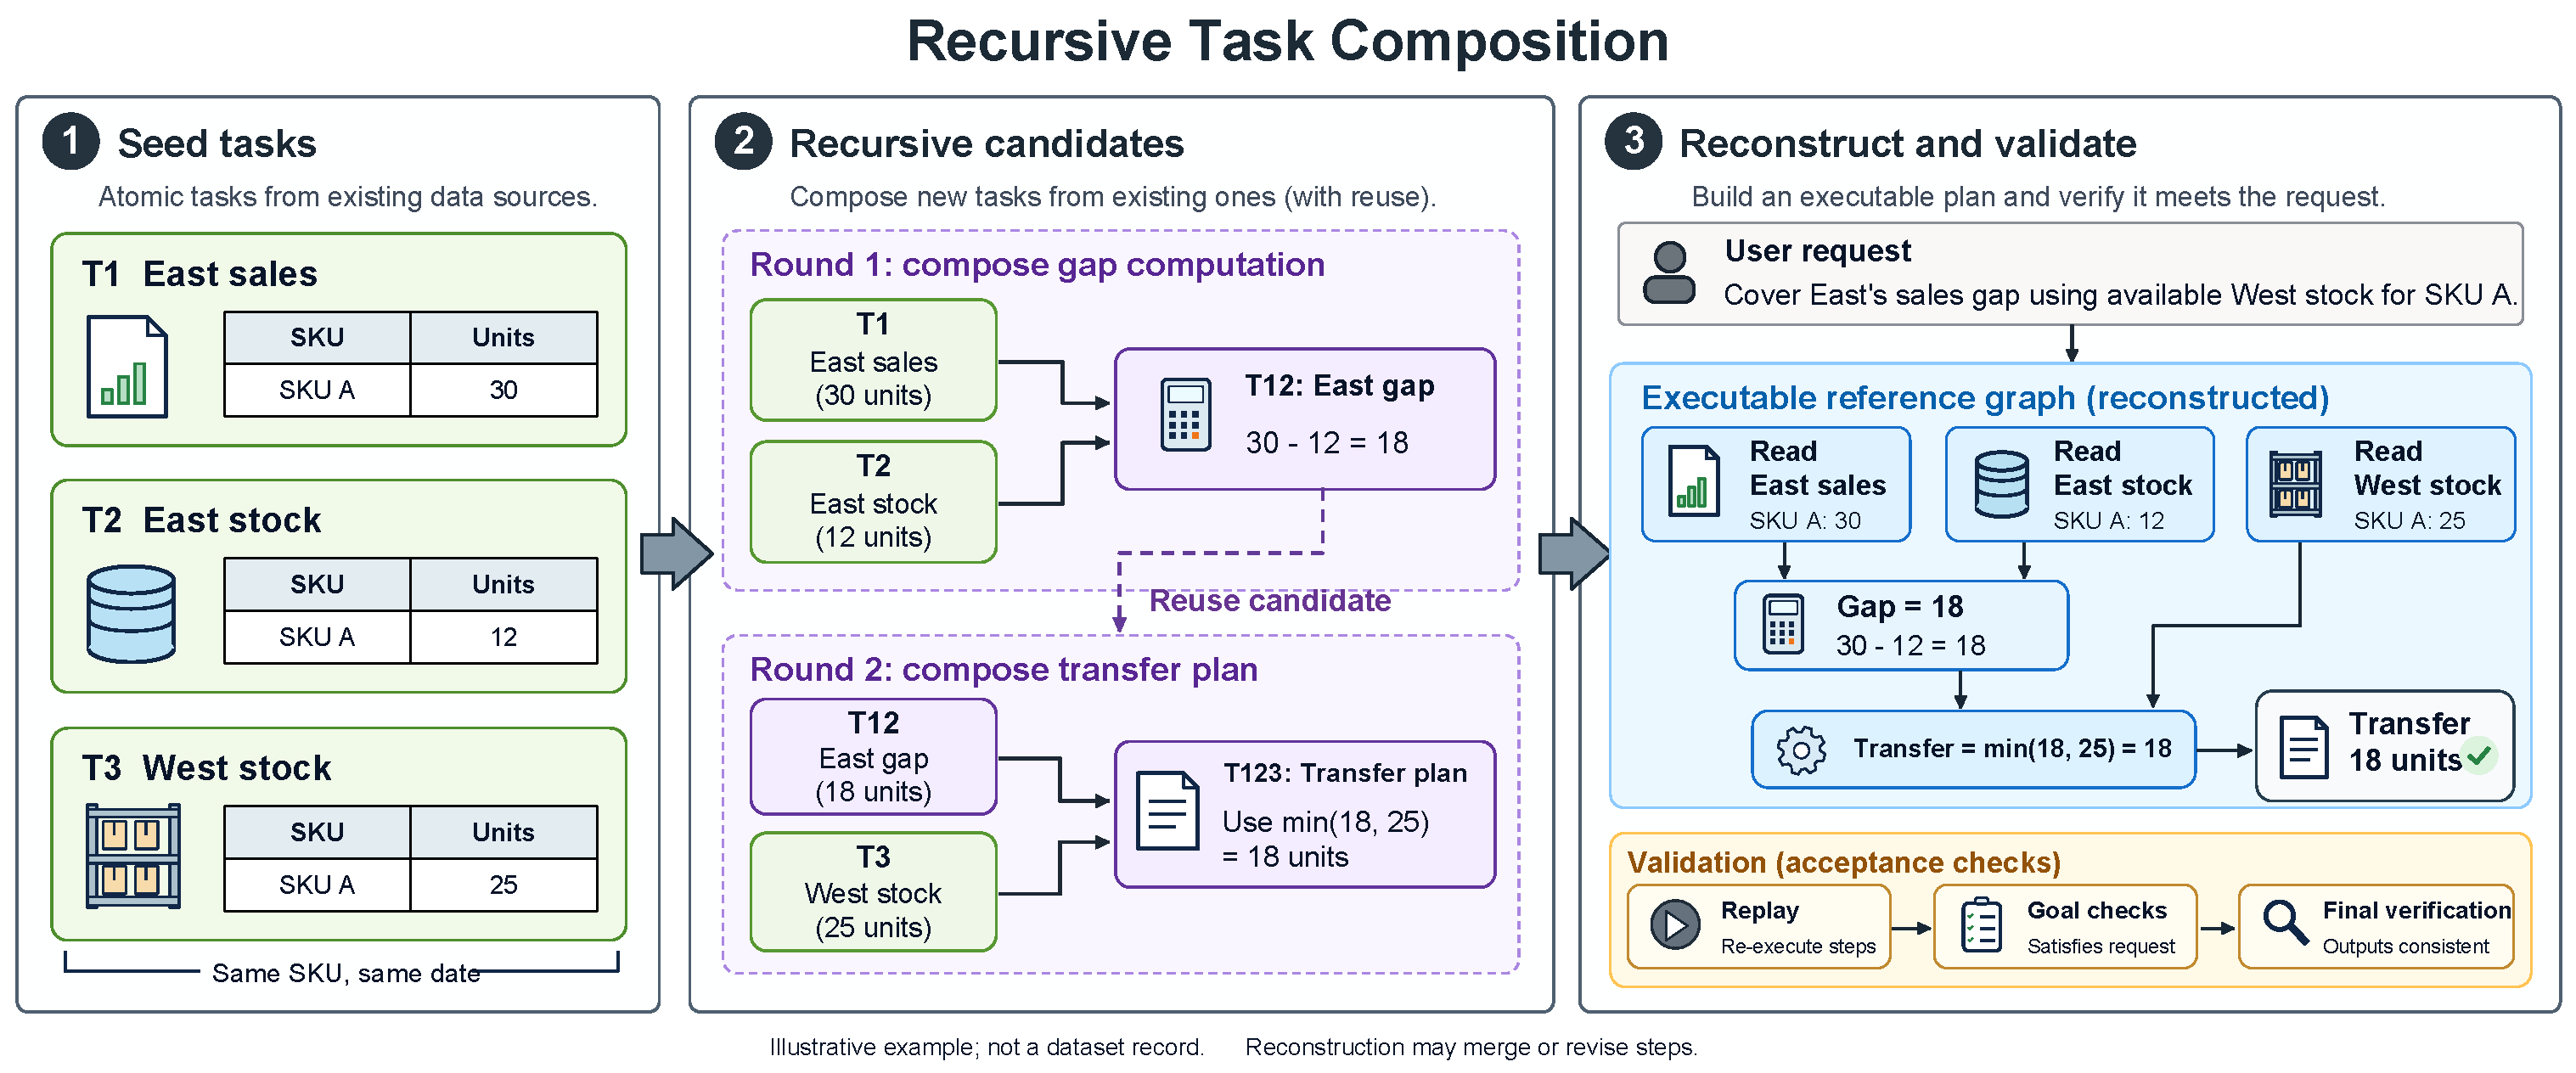
\includegraphics[width=\linewidth]{figures/figure3.pdf}
  \caption{Recursive composition on an illustrative task family. Two rounds of the serial operator turn three atomic seeds into a transfer plan, and reconstruction rebuilds the composed candidate as one executable reference graph that replay and goal checks then validate.}
  \label{fig:composition}
\end{figure}

Figure~\ref{fig:composition} first shows the mechanism on an illustrative task family.
The two cases below show how composition combines parent goals and how reconstruction turns a composed graph into an executable task.
Parent goals and observations are summarized for readability, and the generated request and the reference answer are reproduced in full.

\begin{systembox}{Case 1 \quad Parallel branches over a control plane}
\textbf{Environment.} Control planes with routes and services, and groups of member control planes.

\casepart{Parent tasks and composed graph}
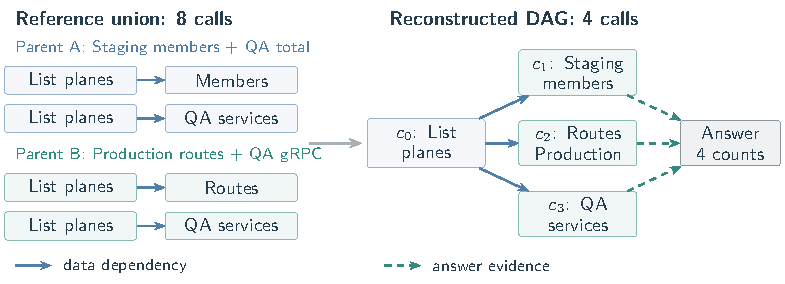
\includegraphics[width=\linewidth]{figures/synthesis_case_kong.pdf}

The two parent graphs form an eight-call reference union. Reconstruction merges the four discovery calls into one and the two service queries into one, and all four requested counts survive.

\casepart{Generated request}
Find the control plane group named 'Staging' and count how many member control planes belong to that group. Then find the control plane named 'Production' with cluster type 'k8s' and count how many routes it has. Next, find the control plane named 'QA' with cluster type 'hybrid' in the 'ap-south' region and count both how many services are deployed to it and how many of those services use the 'grpc' protocol. Return the member count for the Staging group, the route count for Production, the total service count for QA, and the gRPC service count for QA.

\casepart{Reference execution}
\begingroup
\setlength{\tabcolsep}{3pt}\renewcommand{\arraystretch}{1.13}
\begin{tabularx}{\linewidth}{@{}l>{\raggedright\arraybackslash}p{.50\linewidth}Y@{}}
\toprule
 & Tool call & Observation \\
\midrule
$c_0$ & \texttt{list\_control\_planes()} & Staging group 2, Production 1, QA 5. \\
$c_1$ & \texttt{list\_control\_plane\_group\_memberships}\newline\texttt{(groupId=2)} & 2 member planes. \\
$c_2$ & \texttt{list\_routes(controlPlaneId=1)} & 30 routes. \\
$c_3$ & \texttt{list\_services(controlPlaneId=5)} & 10 services, 6 use gRPC. \\
\bottomrule
\end{tabularx}
\endgroup

\casepart{Reference answer and record}
\noindent\begin{minipage}[t]{.60\linewidth}
\vspace{0pt}
\begin{lstlisting}[style=casejson]
{
  "staging_group_member_count": 2,
  "production_route_count": 30,
  "qa_total_service_count": 10,
  "qa_grpc_service_count": 6
}
\end{lstlisting}
\end{minipage}\hfill\begin{minipage}[t]{.36\linewidth}
\vspace{3pt}\raggedright
\textbf{State.} Unchanged.\par\smallskip
\textbf{Independent pairs.} $(c_1,c_2)$, $(c_1,c_3)$, $(c_2,c_3)$, all confirmed by reordered execution.
\end{minipage}
\end{systembox}

\begin{systembox}{Case 2 \quad Serial dependency with pruned calls}
\textbf{Environment.} Documentation sources with crawl, indexing, and search operations.

\casepart{Parent tasks and composed graph}
Parent A refreshes the sources, counts enabled documents, and searches for ``hooks''. Parent B refreshes the same sources, reports enabled documents and index size, and searches for ``error''.

\smallskip
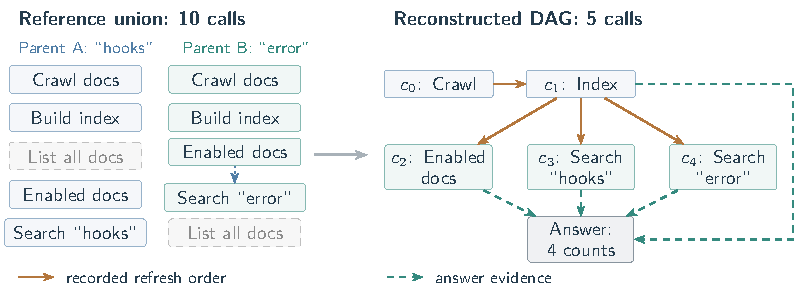
\includegraphics[width=\linewidth]{figures/synthesis_case_docs.pdf}

Reconstruction shares the crawl, the index build, and the enabled-source query, keeps both searches, and removes two listing calls whose outputs support no requested result. The refresh-before-query order is recorded as a state dependency.

\casepart{Generated request}
Refresh the documentation search system by crawling all enabled documentation sources and rebuilding the search index. Then verify the system is working by checking how many documentation sources are currently enabled and indexed, and test the search functionality by querying for both 'hooks' and 'error'. Report the total number of enabled docs, total index entries created, and the number of search results found for each query term.

\casepart{Reference execution}
\begingroup
\setlength{\tabcolsep}{3pt}\renewcommand{\arraystretch}{1.13}
\begin{tabularx}{\linewidth}{@{}l>{\raggedright\arraybackslash}p{.50\linewidth}Y@{}}
\toprule
 & Tool call & Observation \\
\midrule
$c_0$ & \texttt{crawl\_docs()} & Enabled sources crawled. \\
$c_1$ & \texttt{build\_index()} & 10 docs indexed, 224 entries. \\
$c_2$ & \texttt{list\_enabled\_docs()} & 10 docs enabled and indexed. \\
$c_3$ & \texttt{search\_docs(query='hooks')} & 2 matches. \\
$c_4$ & \texttt{search\_docs(query='error')} & 0 matches. \\
\bottomrule
\end{tabularx}
\endgroup

\casepart{Reference answer and record}
\noindent\begin{minipage}[t]{.60\linewidth}
\vspace{0pt}
\begin{lstlisting}[style=casejson]
{
  "enabled_docs_count": 10,
  "index_entries_created": 224,
  "hooks_search_results": 2,
  "error_search_results": 0
}
\end{lstlisting}
\end{minipage}\hfill\begin{minipage}[t]{.36\linewidth}
\vspace{3pt}\raggedright
\textbf{State.} 10 documents updated, 24 pages and 224 index rows added.\par\smallskip
\textbf{Independent pairs.} $(c_2,c_3)$, $(c_2,c_4)$, $(c_3,c_4)$, all after the refresh.
\end{minipage}
\end{systembox}


\section{Dataset Profile and Additional Analyses}
\label{app:stats}



\begin{figure}[ht]
  \centering
  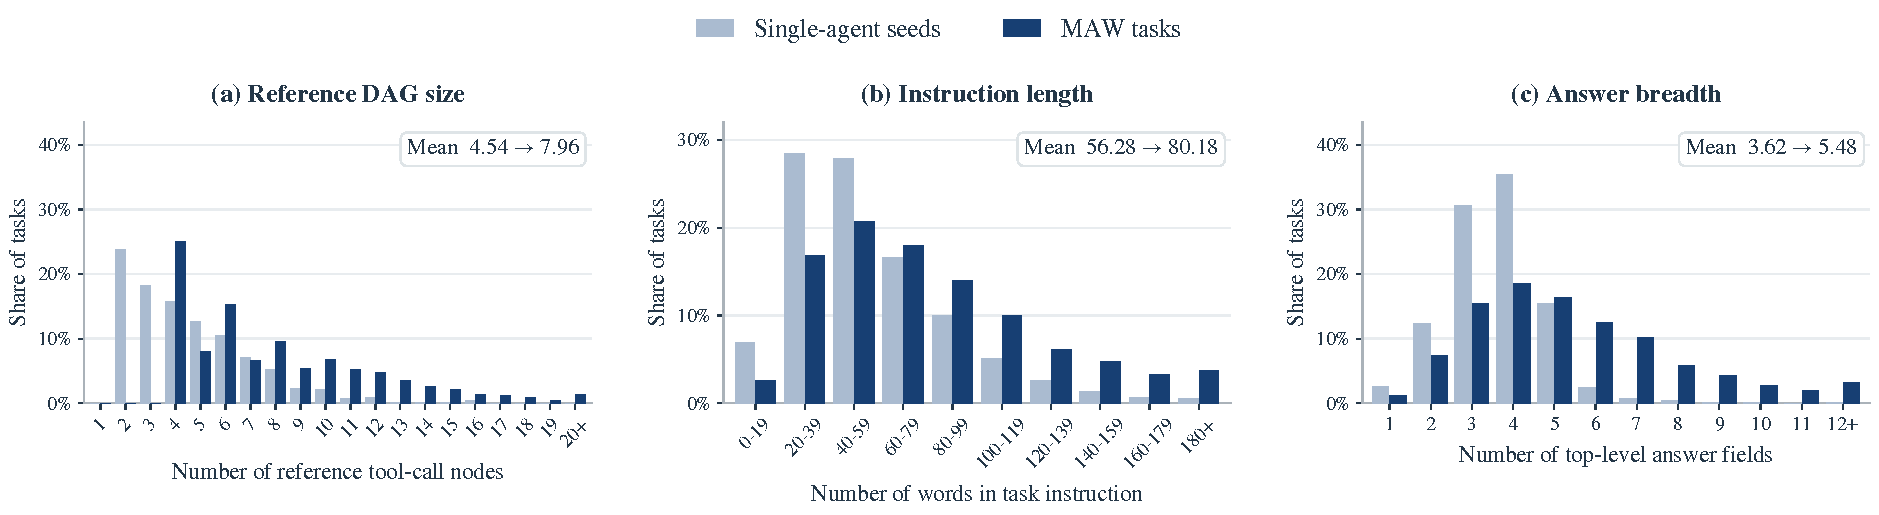
\includegraphics[width=\linewidth]{figures/task_statistics.pdf}
  \caption{Reference structure of the seed pool and of the admitted MAW tasks over 10,860 seeds and 2,581 admitted tasks in 539 environments. Composition grows the number of answer fields far more than the number of tool calls, which indicates that an admitted task asks for more separable results and not simply a longer call chain.}
  \label{fig:task-stats}
\end{figure}

As shown in Figure~\ref{fig:task-stats}, reference tool calls grow by 19.6\% relative to the two parents of each admitted task, distinct tools by 3.9\%, and top-level answer fields by 57.3\%.
The matched baseline of a task is the mean of its two parents, and a parent reused by several descendants contributes once per descendant.

\subsection{Sensitivity, Transfer, and Qualitative Inspection}
\label{app:extra}



\paragraph{Effect of the Process Coefficient and the Schedule Weight.}
\label{sec:sensitivity}

To verify that the reported gains do not depend on a narrow choice of reward weights, we sweep the process coefficient $\lambda$ of Eq.~\ref{eq:reward} and the schedule weight $\alpha_{\mathrm{s}}$ of Eq.~\ref{eq:proc}, keeping every other setting fixed.
The sweep covers the value that removes the process term entirely and values that raise it until process credit approaches the scale of a verified success.

\begin{table}[t]
\centering
\small
\caption{Sensitivity of MAW to the process coefficient $\lambda$ and the schedule weight $\alpha_{\mathrm{s}}$. All rows share the task set, the initialization, and the training budget. The setting used throughout the paper is \colorbox{gray!15}{shaded}.}
\label{tab:sensitivity}
\setlength{\tabcolsep}{6pt}
\renewcommand{\arraystretch}{1.12}
\begin{tabular}{@{}lccc|lccc@{}}
\toprule
$\lambda$ & Success (\%) \up & Goal cov. (\%) \up & $C$ \down & $\alpha_{\mathrm{s}}$ & Success (\%) \up & Goal cov. (\%) \up & $C$ \down \\
\midrule
0.0 & & & & 0.00 & & & \\
0.1 & & & & 0.15 & & & \\
\rowcolor{gray!15}
0.3 & & & & 0.30 & & & \\
0.5 & & & & 0.45 & & & \\
1.0 & & & & 0.60 & & & \\
\bottomrule
\end{tabular}
\end{table}


As shown in Table~\ref{tab:sensitivity}, success is stable across the middle of both ranges and degrades only at the two ends.
A very small $\lambda$ reproduces the outcome-only behavior, and a very large $\lambda$ lets a team collect process credit without finishing the task, which raises goal coverage while success falls.
The schedule weight behaves in the same way, where removing it returns the critical path to the untrained level and raising it too far encourages splitting work that is cheaper to keep together.
The plateau in the middle indicates that the values in Table~\ref{tab:config} were not selected from a narrow optimum.

\paragraph{Generalizability across Worker Backbones.}
\label{sec:worker}

To verify that orchestration training produces a transferable policy and not a policy fitted to one particular worker, we pair the orchestrator trained with frozen Qwen3-8B workers with workers of a different capability at inference and apply no further update.
We keep the interface, the prompts, the budget, and the evaluation instances unchanged, so the only difference is the worker backbone.

\begin{table}[t]
\centering
\small
\caption{Generalization of the trained orchestrator across worker backbones. The orchestrator is trained once with frozen Qwen3-8B workers and then paired with different workers at inference without further updates.}
\label{tab:worker}
\setlength{\tabcolsep}{6pt}
\renewcommand{\arraystretch}{1.12}
\begin{tabular}{@{}llccc@{}}
\toprule
Orchestrator & Workers & Success (\%) \up & $C$ \down & Delivery \up \\
\midrule
Single-agent (init) & Qwen3-8B & & & \\
\rowcolor{gray!15}
MAW & Qwen3-8B & & & \\
Single-agent (init) & Qwen3-14B & & & \\
\rowcolor{gray!15}
MAW & Qwen3-14B & & & \\
\bottomrule
\end{tabular}
\end{table}


As shown in Table~\ref{tab:worker}, MAW improves over the untrained orchestrator under both worker backbones, and the gain in delivery is larger with the weaker workers, where reassignment after an incomplete return matters more.
The critical path shortens under both settings, which indicates that the learned schedule depends on the structure of the request and not on the identity of the worker.
Overall, the results show that the orchestration policy learned in MAW environments carries to teams it was not trained with, which is the property an orchestrator needs in deployment.

\paragraph{Case Study.}
\label{sec:case}

To make the learned behavior concrete, we inspect one successful and one unsuccessful episode from the branch-heavy slice of the held-out set, selected by a fixed sampling rule over the structure of the reference.
In the successful episode, the orchestrator issues one discovery assignment, waits for the identifiers it returns, then assigns three independent lookups in a single concurrent call and merges their results, which matches the dependency and branch pattern that composition wrote into the task.
In the unsuccessful episode, the orchestrator recovers all the branch evidence and drops one of the requested fields when it writes the final answer, which is the integration failure that Eq.~\ref{eq:sched} penalizes and the outcome term alone cannot distinguish from a complete failure.
As shown in Figure~\ref{fig:case}, the two episodes differ only in the final integration step, and the process reward separates them while the outcome term does not.
Appendix~\ref{app:synthesis} provides the full traces, the reference graphs, and the corresponding reward components.

\begin{figure}[t]
  \centering
  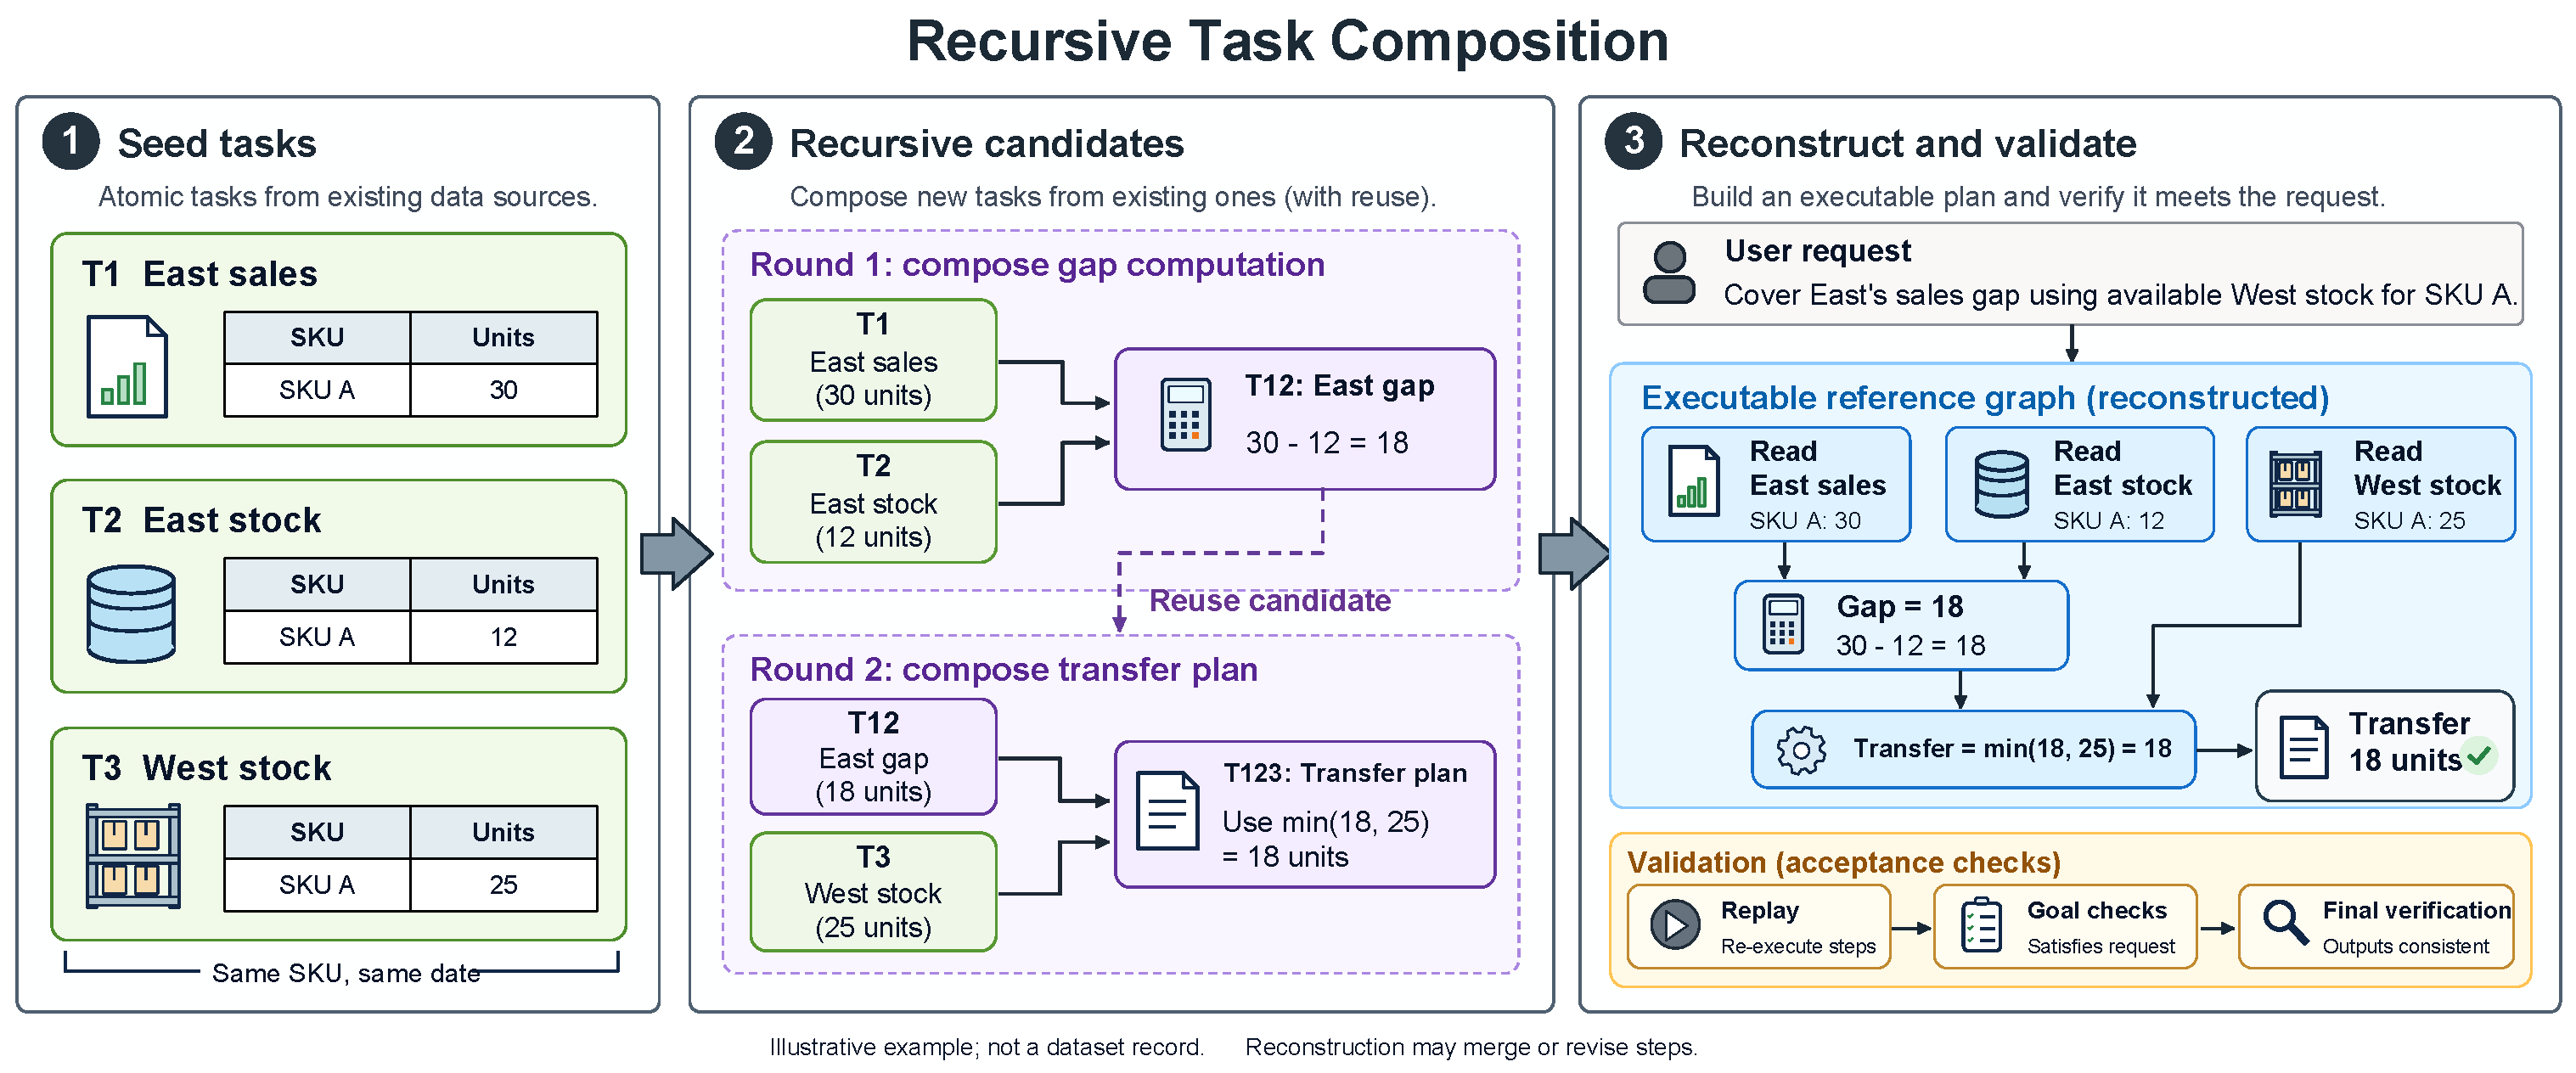
\includegraphics[width=\linewidth]{figures/figure3.pdf}
  \caption{A successful and an unsuccessful episode on the same branch-heavy task. The successful team waits for the discovery result, assigns three independent lookups together, and integrates all of them. The unsuccessful team recovers the same evidence and omits one requested field, which the schedule term penalizes through its integration factor and the outcome term cannot distinguish from a complete failure.}
  \label{fig:case}
\end{figure}

\section{Multi-Agent Runtime and Information Boundary}
\label{app:runtime}

Table~\ref{tab:actions} lists the four actions of the delegation-only harness.

\begin{table}[ht]
\centering\small
\caption{Orchestration interface. A worker is registered with a role and a permitted tool subset, a single assignment is synchronous, and a batch assignment launches workers concurrently and returns when their results join.}
\label{tab:actions}
\begin{tabularx}{\linewidth}{lY}
\toprule
Action & Required information and effect \\
\midrule
\texttt{create\_subagent} & Name, system prompt, and allowed tool names, which registers a worker that follows the frozen policy. \\
\texttt{assign\_task} & Worker name and subtask prompt, which executes one assignment and returns its result. \\
\texttt{assign\_tasks} & A list of assignments, which permits concurrent worker inference and joins the returns. \\
\texttt{submit\_answer} & The final answer in the required format, which triggers completion and verification. \\
\bottomrule
\end{tabularx}
\end{table}

Worker reasoning can overlap, and tool operations on the database commit under a transaction lock, so a concurrent assignment never produces an interleaving that the environment cannot reproduce.
Table~\ref{tab:visibility} states which information each participant can access during an episode.
The reference plan, the expected answer, and the reward components are available only to the reward service, and no reward report is returned to the policy as an observation.
A leakage audit inspects the rendered requests and tool descriptions of the training and evaluation manifests for reference answers, serialized reference graphs, and verifier diagnostics, and tasks descending from the same seed family are grouped before any split.

\begin{table}[ht]
\centering\small
\caption{Information boundary during an episode. Reward reports are never returned as observations, so the policy cannot read its own process score.}
\label{tab:visibility}
\begin{tabularx}{\linewidth}{Yccc}
\toprule
Information & Orchestrator & Worker & Reward service \\
\midrule
User request & Yes & Assigned content & Yes \\
Allowed tool descriptions & Yes & Permitted subset & Yes \\
Tool and worker returns & Returned content & Own context & Logged content \\
Reference plan and expected answer & No & No & Yes \\
Independence record $\Pi$ & No & No & Yes \\
Reward component scores & No & No & Yes \\
\bottomrule
\end{tabularx}
\end{table}

\paragraph{Critical-path Reconstruction.}
Execution cost is a diagnostic and is not part of Eq.~\ref{eq:reward}.
Let $w(v)=1$ for each orchestrator or worker generation event and zero otherwise.
Retaining only causal parents, the depth of an event and the cost of an episode are
\begin{equation}
d(v)=w(v)+\max_{u\in\mathrm{pa}(v)}d(u),\qquad C(\tau)=\max_{v\in G_\tau}d(v),
\label{eq:critical-path}
\end{equation}
where an empty maximum is zero and edges that represent only the serialized commit order are excluded.
For a fork and join execution in which one orchestrator generation precedes two worker branches of length three and five and one integration generation follows, the critical path is $1+\max(3,5)+1=7$ model rounds while serial execution of the same ten generations gives $10$.

\section{Reward Computation}
\label{app:process}

\paragraph{Tool and Answer Matching.}
A reference milestone specifies a tool, its arguments, and the expected observation.
Arguments are compared after declared defaults are filled and after the environment-specific normalization rules listed in the task package are applied, and observations are canonicalized and hashed.
Only successful events contribute coverage, and each milestone is credited once, so repeated calls do not raise $f_{\mathrm{tool}}$.
The answer term is $f_{\mathrm{ans}}(\tau)=\tfrac{m}{n^{\star}}(0.8+0.2\tfrac{m}{n})$, where $n^{\star}$ and $n$ are the reference and submitted field counts and $m$ is the matched count, so recall carries most of the weight and the precision factor removes any gain from padding.
Scalar and structured values require equality, and list elements are matched one to one without reuse.

\paragraph{Delivery and Schedule.}
Each credited subtask has one assignment owner, and a repeated or empty instruction receives no ownership.
Delivery checks whether the worker return contains the required raw evidence or a matching derived result, which is stricter than a claim of completion.
For $f_{\mathrm{sch}}$, a pair in $\Pi$ counts toward $\Pi_\tau$ when the two subtasks are owned by different workers and the assignment intervals are causally independent, so issuing two assignments in sequence and waiting for the first does not count as parallel scheduling.
Tasks with an empty $\Pi$ fall back to a conservative schedule score based on covered milestones, satisfied dependencies, and non-redundant assignments.

\paragraph{Outcome Priority.}
Under Eq.~\ref{eq:reward}, a successful team satisfies $f_{\mathrm{out}}=1$ and $f_{\mathrm{proc}}\ge 0$, which gives $R\ge 1$, and an unsuccessful team satisfies $f_{\mathrm{out}}=0$ and $f_{\mathrm{proc}}\le 1$, which gives $R\le\lambda$.
Every verified success therefore outranks every failure, and the property assumes a correct outcome checker and bounded process terms.

\section{Training and Evaluation Configuration}
\label{app:training}

\begin{table}[ht]
\centering\small
\caption{Training configuration of MAW. The orchestrator and the workers start from the same single-agent checkpoint, and only the orchestrator is updated.}
\label{tab:config}
\begin{tabularx}{\linewidth}{YY}
\toprule
Setting & Value \\
\midrule
Backbone & Qwen3-8B \\
Orchestrator initialization & Single-agent checkpoint \\
Worker initialization and update & Same checkpoint, frozen \\
Optimization & GRPO with outcome and process reward \\
Rollouts per task & 8 \\
Process coefficient $\lambda$ & 0.3 \\
Process weights $(\alpha_{\mathrm t},\alpha_{\mathrm a},\alpha_{\mathrm d},\alpha_{\mathrm s})$ & $(0.25,0.25,0.20,0.30)$ \\
Cost in the training reward & None \\
Completion protocol & At least one delegation \\
\bottomrule
\end{tabularx}
\end{table}

Every benchmark is evaluated with a frozen dataset revision, evaluator commit, subset manifest, and decoding configuration, and function-calling accuracy and task success are reported in separate columns with no average across heterogeneous metrics.
The primary unit of analysis is the task, every method attempts the same instances under paired seeds, and uncertainty is estimated with paired bootstrap resampling of task identifiers.
Infrastructure failures such as an unavailable service are logged separately from a valid trajectory that fails verification, and a rerun uses the same inputs and is counted in the run ledger.
Benchmark tasks and benchmark-derived references are excluded from synthesis, from reward annotation, and from model selection.

\section{Statements}
\label{app:statements}

\paragraph{Reproducibility.}
The research package contains the environment and reset manifests, the task provenance and independence records, the synthesis and admission code, the reward implementation, the prompts, the baseline adapters, the training configurations, and the per-task evaluation logs.
Hidden references are stored separately from the assets visible to a solver.

\paragraph{Ethics.}
Synthetic tool environments can encode unrealistic assumptions or faulty checks, so they are executed in isolated sandboxes and reviewed for copied private data, credential-like strings, and unauthorized external effects before release.
The same orchestration capability that distributes useful work can distribute harmful actions, so deployment requires tool-level permissions and monitoring beyond the training reward.


\end{document}
